\documentclass[a4paper]{article}
\usepackage{graphicx}
\usepackage[utf8]{inputenc}
\usepackage[english, serbian]{babel}
\usepackage{comment}
\usepackage[unicode]{hyperref}
\hypersetup{colorlinks,citecolor=green,filecolor=green,linkcolor=blue,urlcolor=blue}
\usepackage{cleveref}
\usepackage[a4paper, total={6in, 8in}]{geometry}
\usepackage{datetime}
\usepackage{rotating}
\usepackage{afterpage}

\newdateformat{mydate}{\THEDAY. \monthname[\THEMONTH] \THEYEAR.}

\begin{document}
\begin{titlepage}

\newcommand{\HRule}{\rule{\linewidth}{0.5mm}} % Defines a new command for the horizontal lines, change thickness here

\center % Center everything on the page
 
%----------------------------------------------------------------------------------------
%	HEADING SECTIONS
%----------------------------------------------------------------------------------------

\textsc{\LARGE Matematički fakultet}\\[1.5cm] % Name of your university/college
\textsc{\Large Projekat iz predmeta Informacioni sistemi}\\[0.5cm] % Major heading such as course name
\textsc{\large Školska 2018/2019.}\\[0.5cm] % Minor heading such as course title

%----------------------------------------------------------------------------------------
%	TITLE SECTION
%----------------------------------------------------------------------------------------

\HRule \\[0.4cm]
{ \huge \bfseries MATF Časopis}\\[0.4cm] % Title of your document
\HRule \\[1.5cm]
 
%----------------------------------------------------------------------------------------
%	AUTHOR SECTION
%----------------------------------------------------------------------------------------

\begin{minipage}{0.4\textwidth}
\begin{flushleft} \large
\emph{Autori:}\\
Dimitrije \textsc{Špadijer}\\
Božidar \textsc{Antić}\\
Nadežda \textsc{Bogdanović}
\end{flushleft}
\end{minipage}
~
\begin{minipage}{0.4\textwidth}
\begin{flushright} \large
\emph{Predavači:} \\
dr Saša \textsc{Malkov}\\
Aleksandra \textsc{Kocić}
\end{flushright}
\end{minipage}\\[2cm]

% If you don't want a supervisor, uncomment the two lines below and remove the section above
%\Large \emph{Author:}\\
%John \textsc{Smith}\\[3cm] % Your name

%----------------------------------------------------------------------------------------
%	DATE SECTION
%----------------------------------------------------------------------------------------
\mydate
{\large \today}\\[2cm] % Date, change the \today to a set date if you want to be precise

%----------------------------------------------------------------------------------------
%	LOGO SECTION
%----------------------------------------------------------------------------------------


\includegraphics[width=40mm]{logo.jpg}\\[1cm] % Include a department/university logo - this will require the graphicx package
 
%----------------------------------------------------------------------------------------

\vfill % Fill the rest of the page with whitespace

\end{titlepage}


\tableofcontents
\newpage

\section{Cilj projekta}
\label{section:ciljprojekta}

Cilj projekta je razviti web platformu koja će omogućiti sve neophodne funkcionalnosti za uređivanje elektronskog časopisa. Jezik časopisa je engleski i tematski je organizovan.

Radi boljeg razumevanja projekta, sam dokument je podeljen na 4 tematske celine: \textbf{Analiza sistema}, \textbf{Slučajevi upotrebe}, \textbf{Model baze podataka} i \textbf{Arhitektura sistema}.

Javni repozitorijum projekta se nalazi na: \url{https://github.com/Nacili/MATFCasopis}

Sistem je, sa određenim izmenama, projektovan na osnovu dokumenta \cite{ecas} primljenog od naručioca.

\newpage

\section{Analiza sistema}
\label{section:analiza}

U ovom odeljku biće prikazana podela sistema na \textbf{module}: \textit{Učesnici}, \textit{Izdanje časopisa} i \textit{Rad}, kao i opis samih modula. Ostvarivanje njihovih zahteva i specifikacije biće prikazane u odeljku \ref{section:slucajeviupotrebe}. Opšti pogled na sistem prikazan je dijagramom konteksta na slici \ref{fig:konteksta}
\begin{figure}[hbt!]
    \begin{center}
    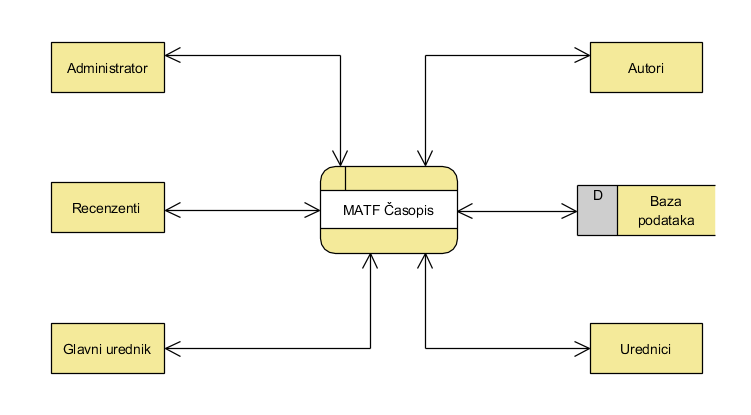
\includegraphics[width=1\linewidth]{Konteksta.PNG}
    \end{center}
    \caption{Dijagram konteksta \cite{smalkov} \cite{vparadigm}}
    \label{fig:konteksta}
\end{figure}

\subsection{Učesnici}
\label{subsection:ucesnici}
    
    Učesnici se dele u 5 korisničkih grupa, koje se međusobno razlikuju po \textit{ulogama}, a samim tim i \textit{privilegijama}\footnote{ Privilegija je posao koji korisnik može da obavlja na sistemu} koje su im dodeljene. Za razliku od ostalih, uloge \textit{Administrator} i \textit{Glavni urednik} mogu biti dodeljene samo jednom korisniku. Osnovna uloga, koja obezbeđuje i privilegije zajedničke svim ostalim korisnicima (sem administratoru) je \textit{Autor}.
    
   \subsubsection{Autor}
   \label{subsubsection:autor}
    Osnovne privilegije:
    \begin{itemize}
        \item Registracija
        \item Logovanje
        \item Odjava
        \item Promena sopstvenih podataka
        \item Komunikacija sa ostalim korisnicicma
        \item Prijava rada
        \item Ažuriranje rada (ostvaruje se kroz prijavu nove verzije istog rada)
        \item Povlačenje rada
    \end{itemize}
    
    \subsubsection{Recenzent}
    \label{subsubsection:recenzent}
     Potencijalni recenzent je onaj koji je već recenzirao neki rad, ili  neko ko je  prilikom registracije čekirao polje "nemam ništa protiv da me kontaktirate za recenziranje nekog rada". Isto ovo polje može da čekira i kasnije, na svojoj korisničkoj stranici.
     
    Dodatne privilegije:
    \begin{itemize}
        \item Odbijanje recenziranja rada
        \item Pregled svih radova za koje je prihvaćena recenzija
        \item Ostavljanje recenzije na rad (ostvaruje se ostavljanjem recenzije na verziju rada)
    \end{itemize}
    
    \subsubsection{Urednik}
    \label{subsubsection:urednik}
    Dodatne privilegje:
    \begin{itemize}
        \item Slanje predloga za recenziranje
        \item Odbacivanje rada
        \item Prihvatanje rada
        \item Komentarisanje rada
    \end{itemize}
    
    \subsubsection{Glavni urednik}
    \label{subsubsection:glavniurednik}
    Ne registruje se u sistem, već ga sam administrator dodaje. Nalazi se na vrhu piramide odlučivanja: ako je urednik odlučio da se rad prihvata/odbacuje, glavni urednik može tu odluku da promeni i njegova odluka je konačna.
    Dodatne privilegije:
     \begin{itemize}
         \item Prihvatanje rada
         \item Odbacivanje rada
         \item Ostavljanje komentara na rad
         \item Dodela uloga korisnicima
         \item Upravljanje izdanjem časopisa (odlučivanje o tome koji će se rad naći u kojem broju, minimalan i maksimalan broj radova po izdanju...)
     \end{itemize}
    
    \subsubsection{Administrator}
    \label{subsubsection:administrator}
    On se odmah od početka korišćenja sistema nalazi u bazi podataka - ne registruje se.
    Posebne privilegije:
    \begin{itemize}
        \item Upravljanje podešavanjima sistema (promena podataka samom časopisu i ostale stvari tehnološke prirode)
        \item Upravljanje podešavanjima korisnika (promena korisničkih imena, šifri, dodavanje glavnog urednik u sistem...)
    \end{itemize}
    
\subsection{Izdanje časopisa}
\label{section:izdanjecasopisa}
Izdanje predstavlja broj jednog časopisa i može biti zimsko i letnje. Glavni urednik odlučuje koji će se radovi u njemu naći i u kom redosledu, koliko će ih biti i koji naslov će tekući broj da nosi.

\subsection{Rad}
\label{subsection:rad}
    Statusi rada koji ujedno opisuju i njegov životni ciklus prikazana su na slici \ref{fig:stanjarada}:
    \begin{figure}[ht!]
    \begin{center}
    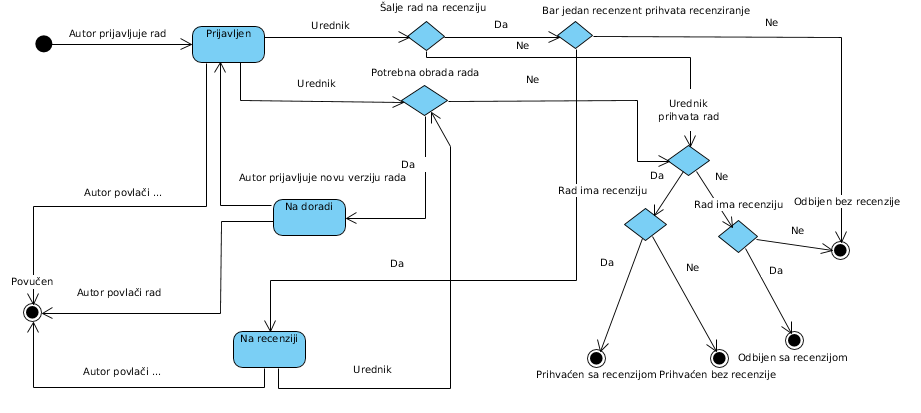
\includegraphics[width=1.1\linewidth]{StanjeRada.PNG}
    \end{center}
    \caption{Stanja rada \cite{alex} \cite{vparadigm}}
    \label{fig:stanjarada}
    \end{figure}
    \begin{itemize}
        \item prijavljen: rad može imati više autora, ali ga samo jedan od njih prijavljuje i smatra se odgovornim licem za taj rad. Prilikom prijavljivanja rada, autor popunjava formular u kojem navodi i ostale autore, koji se, ako već nisu registrovani, dodaju u sistem.
        \item prihvaćen bez recenzije: (glavni) urednik je odlučio da prihvata rad bez konsultacije sa recenzentima. U tom slučaju je dužan da ostavi komentar na rad.
        \item odbijen bez recenzije: (glavni) urednik je odlučio da odbije rad bez konsultacije sa recenzentima, nakon čega ostavlja komentar na rad. Rad može dobiti ovaj status i ako ni jedan recenzent ne želi da ga recenzira.
        \item na recenziji: urednik označi recenzente za rad i status rada automatski postaje "na recenziji"
        \item na doradi: ovaj status dobija kada  (glavni) urednik označi da rad treba da ide na doradu, bez obzira na to da li je pre toga bio na recenziji ili ne. Ako je rad pre dorade bio na recenziji, poželjno je i da na recenziju ide nakon obrade i da mu se dodele pređašnji recenzenti
        \item povučen: autor je podneo zahtev za povlačenje rada
        \item odbijen sa recenzijom: (glavni) urednik je nakon recenziranja odlučio da se rad odbije
        \item prihvaćen sa recenzijom: (glavni) urednik je nakon recenzije odlučio da prihvati rad
    \end{itemize}
    
\newpage

\section{Slučajevi upotrebe}
\label{section:slucajeviupotrebe}
Ovaj odeljak pruža detaljan opis načina na koji se sistem koristi. Glavni procesi koji se u njemu izdvajaju su prikazani na slici \ref{fig:nivo0}:
\begin{figure}[h!]
   \begin{center}
    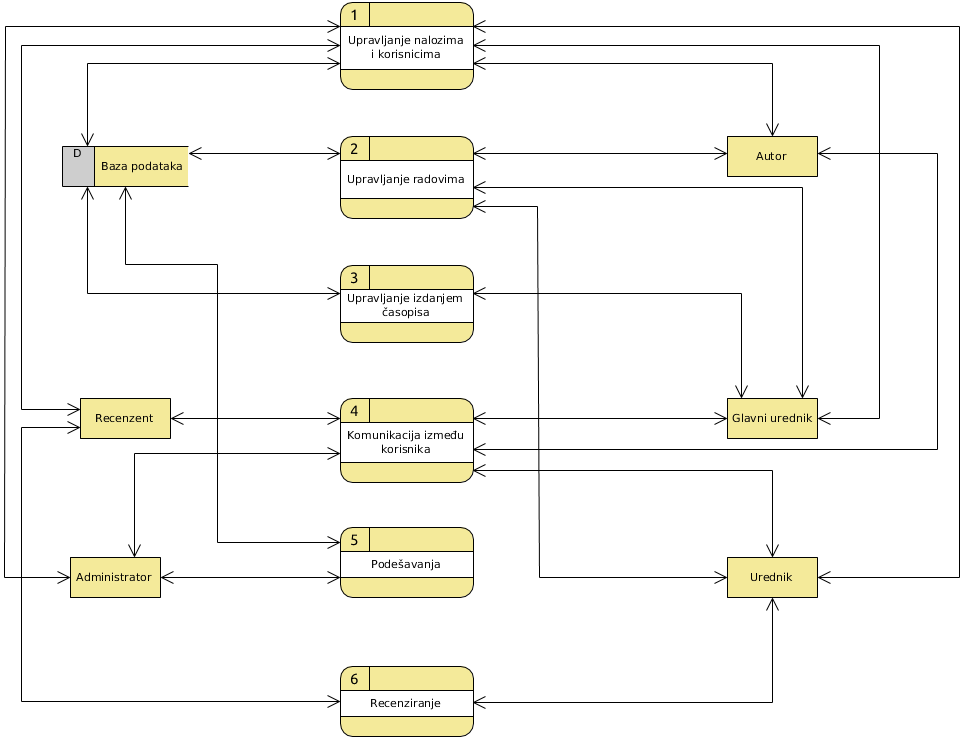
\includegraphics[width=1.15\linewidth]{Nivo0.png}
    \end{center}
    \caption{Dijagram toka podataka nivoa 0 \cite{smalkov} \cite{vparadigm}}
    \label{fig:nivo0}
\end{figure}

%ovde treba da stoji slika

\subsection{Upravljanje nalozima i korisnicima}
\label{subsection:upravljanjenalozimaikorisnicimasec}
Kao što je prikazano na slici \ref{fig:upravljanjenalozimaikorisnicima}, proces obuhvata sledeće slučajeve upotrebe: \textit{registracija korisnika}, \textit{prijavljivanje korisnika}, \textit{odjava korisnika}, \textit{promena ličnih podataka}, \textit{promena korisničkih podataka}, \textit{dodela/oduzimanje uloga korisnicima}.
\begin{figure}[h!]
    \centering
    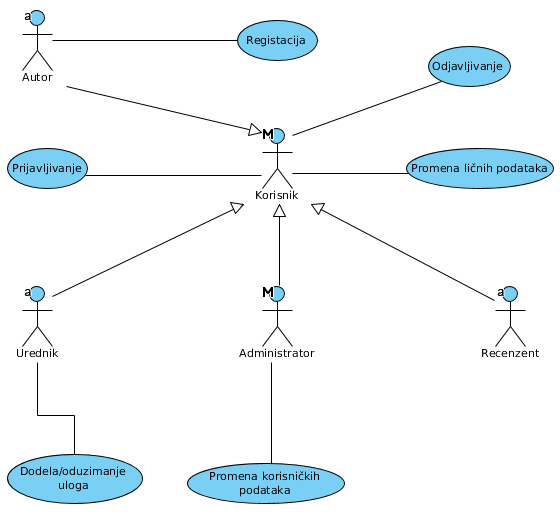
\includegraphics[width=0.9\linewidth]{UpravljanjeNalozimaIKorisnicima.PNG}
    \caption{Upravljanje nalozima i korisnicima \cite{alex} \cite{vparadigm}}
    \label{fig:upravljanjenalozimaikorisnicima}
\end{figure}

\subsubsection{Registracija korisnika}
\label{subsubsection:registracijakorisnikasec}
\begin{itemize}
    \item Akter: Korisnik
    \item Kratak opis: Korisnik unosi potrebne podatke kako bi se registrovao u sistemu
    \item Preduslov: Korisnik nije već registrovan
    \item Postuslov: Novi korisnik je dodat u sistem
    \item Osnovni tok događaja:
        \begin{enumerate}
            \item Korisnik unosi podatke u formular koji mu se prikazuje nakon zahteva za registracijom
            \item Korisnik pokušava da se registruje
            \item Sistem prikazuje narednu stranicu za potvrdu email adrese
            \item Korisnik potvrđuje svoju email adresu
            \item Sistem uspešno registruje korisnika
        \end{enumerate}
    \item Alternativni tok događaja:
        \begin{enumerate}
            \item Neko od obaveznih polja nije popunjeno
                \begin{enumerate}
                    \item Nakon 2. koraka sistem ispisuje poruku o grešci i zahteva od korisnika da unese podatke koji fale u obaveznim poljima i ta polja bivaju označena.
                    \item Korisnik popunjava tražena polja.
                    \item Korisnik zatim ponavlja korak 2 iz osnovnog toka.
                \end{enumerate}
            \item Vrednosti u poljiva Confirm email i Repeat Password ne odgovaraju vrednostima u poljima Email i Password
                \begin{enumerate}
                    \item Nakon 2. koraka sistem ispisuje poruku o grešci i obaveštava korisnika o nepoklapanju podataka u datim poljima.
                    \item Korisnik ponovo popunjava sporna polja.
                    \item Korisnik zatim ponavlja korak 2 iz osnovnog toka.
                \end{enumerate}
            \item Neko od polja ne odgovara formatu koji je za to polje zadat regularnim izrazom
                \begin{enumerate}
                    \item Nakon 2. koraka sistem ispisuje poruku o grešci i zahteva od korisnika da unese podatke u odgovarajućem formatu za polja koja označava na neki način.
                    \item Korisnik ponovo popunjava tražena polja.
                    \item Korisnik zatim ponavlja korak 2 iz osnovnog toka.
                \end{enumerate}
        \end{enumerate}
        \item Dodatak: slike \ref{fig:registracijakorisnika} i \ref{fig:registracijakorisnikaforma}

\begin{figure}[ht!]
    \centering
    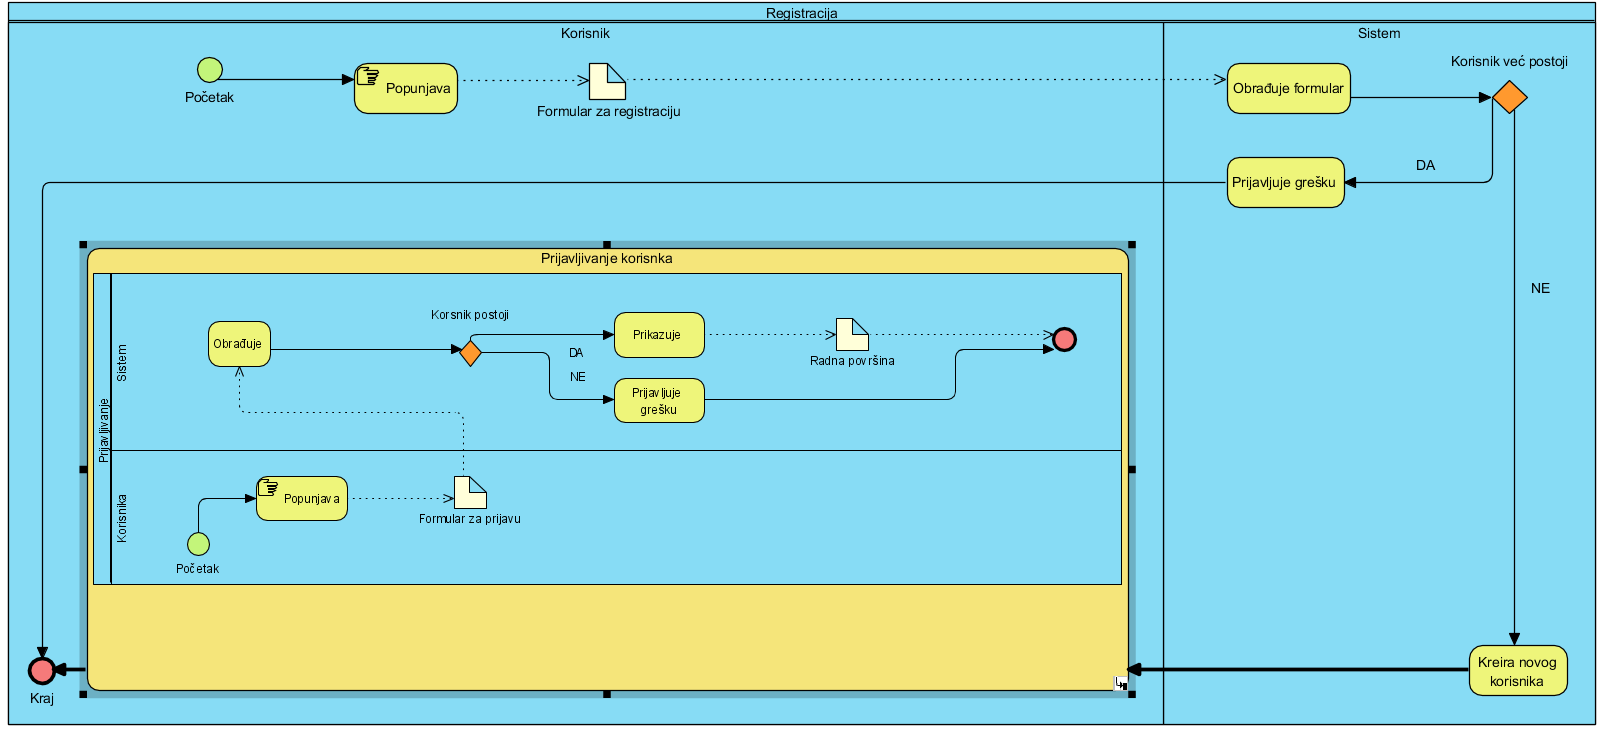
\includegraphics[width=1.15\linewidth]{RegistracijaKorisnika.PNG}
    \caption{Registracija korisnika \cite{smalkov} \cite{vparadigm}}
    \label{fig:registracijakorisnika}
\end{figure}
%\afterpage{\clearpage}
%\begin{sidewaysfigure}[ht!]
%    \centering
%    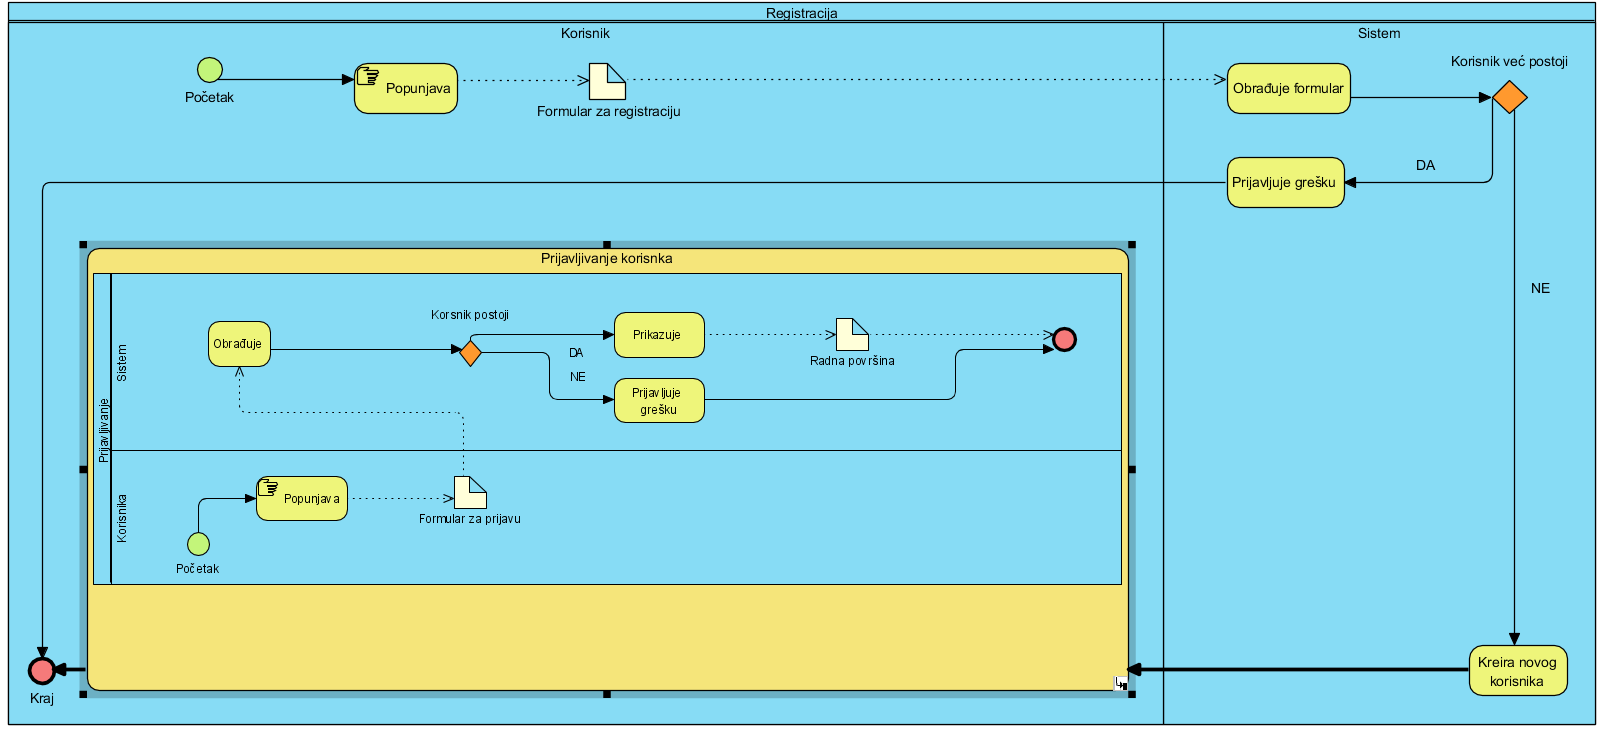
\includegraphics[width=1\linewidth]{RegistracijaKorisnika.PNG}
%    \caption{Registracija korisnika}
%    \label{fig:registracijakorisnika}
%\end{sidewaysfigure}
\begin{figure}[ht!]
    \centering
    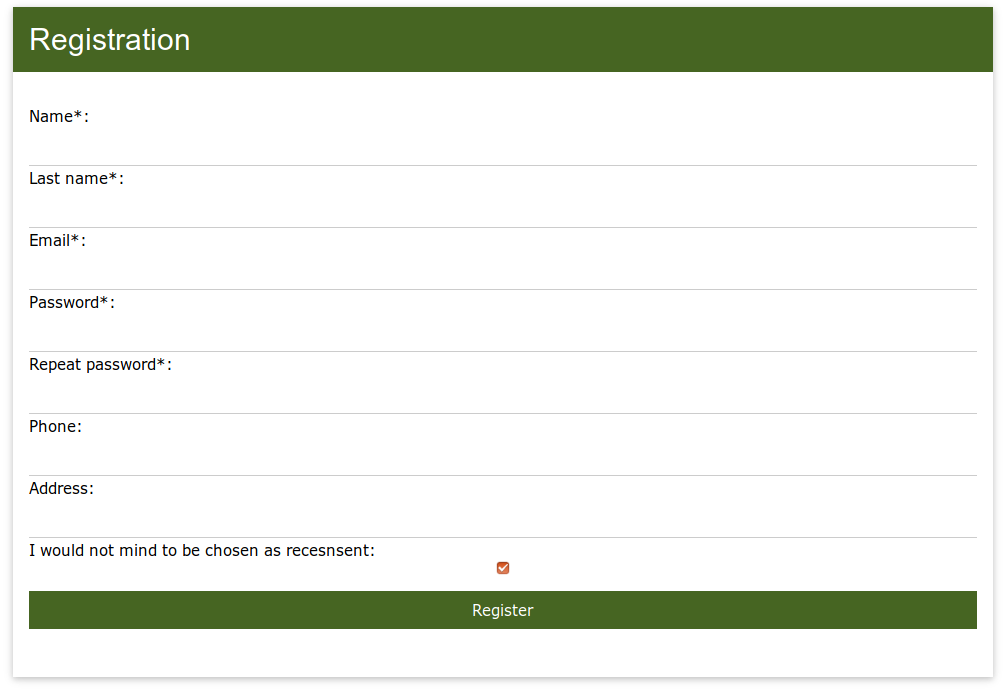
\includegraphics[width=1\linewidth]{Register.png}
    \caption{Registracija korisnika forma}
    \label{fig:registracijakorisnikaforma}
\end{figure}

% U okviru ovog slučaja upotrebe treba da stoje slike

\end{itemize}

\newpage

\subsubsection{Prijavljivanje korisnika}
\label{subsubsection:prijavljivanjekorisnika}
\begin{itemize}
    \item Akter: Korisnik
    \item Kratak opis: Korisnik unosi potrebne podatke kako bi se ulogovao u sistem
    \item Preduslovi: Korisnik postoji u sistemu
    \item Postuslovi: Nema
    \item Osnovni tok događaja:
        \begin{enumerate}
            \item Korisnik unosi svoju email adresu i šifru u polja koja su za to predoređena
            \item Korisnik šalje sistemu zahtev za prijavu
            \item Sistem autentifikuje korisnika
            \item Sistem prikazuje korisniku početnu stranicu
        \end{enumerate}
    \item Alternativni tok događaja:
        \begin{enumerate}
            \item Autentifikacija korisnika nije uspela zbog neispravno unetih podataka
                \begin{enumerate}
                    \item Nakon 2. koraka osnovnog toka, sistem ispisuje poruku o neuspešnoj autentikaciji zbog neispravno unetih podataka.
                    \item Korisnik ponavlja korake 1. i 2. osnovnog toka.
                \end{enumerate}
            \item Autentifikacija korisnika nije uspela zbog greške u sistemu
                \begin{enumerate}
                    \item Nakon 2. koraka osnovnog toka, sistem ispisuje poruku o neuspešnoj autentifikaciji zbog greške u sistemu
                    \item Korisnik obaveštava administratora časopisa o postojanju tehničkih problema u sistemu.
                \end{enumerate}
        \end{enumerate}
        \item Dodatak: slika \ref{fig:registracijakorisnika}
\end{itemize}

\subsubsection{Odjavljivanje korisnika}
\label{subsubsection:odjavljivanjekorisnika}
\begin{itemize}
    \item Akter: Korisnik
    \item Kratak opis: Korisnik se odjavljuje iz sistema
    \item Preduslovi: Korisnik postoji u sistemu i prijavljen je
    \item Postuslovi: Nema
    \item Osnovni tok događaja:
        \begin{enumerate}
            \item Korisnik šalje zahtev sistemu da ga odjavi
            \item Sistem odjavljuje korisnika
            \item Sistem prikazuje korisniku početnu stranicu
        \end{enumerate}
\end{itemize}

\newpage

\subsubsection{Dodela/Oduzimanje uloga korisnicima}
\label{subsubsection:ulogesec}
\begin{itemize}
    \item Akter: Glavni urednik
    \item Kratak opis: Glavni urednik časopisa dodeljuje/oduzima recenzentsku ili uredničku ulogu postojećem korisniku sistema.
    \item Preduslovi: Postoje korisnici sistema koji nemaju ulogu recenzenta ili urednika. Korisnik kojem glavni urednik želi da dodeli ulogu recenzenta je označio da nema ništa protiv da mu bude dodeljena uloga recenzenta. 
    \item Postuslovi: Nema
    \item Osnovni tok događaja:
        \begin{enumerate}
            \item Glavni urednik upućuje upit sistemu za spisak svih korisnika sistema.
            \item Sistem vraća spisak svih korisnika sistema.
            \item Glavni urednik bira korisnika sistema.
            \item Glavni urednik dodeljuje/oduzima ulogu recenzenta ili urednika korisniku sistema.
            \item Sistem čuva izmene o ulozi korisnika.\\
            Ponavljati korake 3, 4 i 5 dok za tim ima potrebe.
        \end{enumerate}
    \item Alternativni tok događaja:
        \begin{enumerate}
            \item Sistem ne vraća uspešno spisak korisnika sistema.
            \begin{enumerate}
                \item U 2. koraku osnovnog toka, sistem ne vraća uspešno spisak korisnika sistema i obaveštava glavnog urednika o grešci.
                \item Glavni urednik se vraća na 1. korak osnovnog toka ili se obraća administratoru.
            \end{enumerate}
            \item Sistem ne čuva izmene o ulozi korisnika.
            \begin{enumerate}
                \item U 5. koraku osnovnog toka, sistem ne čuva izmene o ulozi korisnika i obaveštava glavnog urednika o grešci.
                \item Glavni urednik se vraća na 4. korak osnovnog toka ili se obraća administratoru.
            \end{enumerate}
        \end{enumerate}
        \item Dodatak: slika \ref{fig:uloge}
\begin{figure}[ht!]
    \centering
    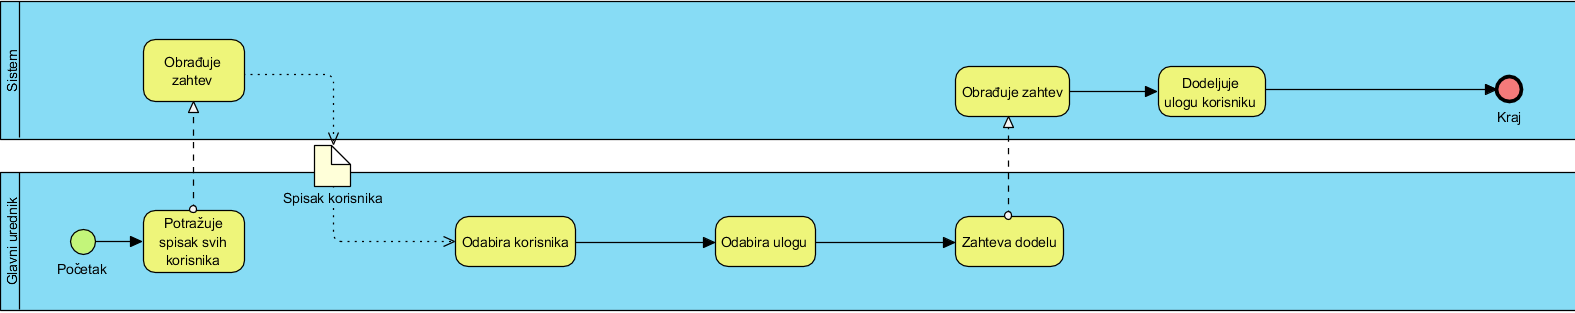
\includegraphics[width=1.15\linewidth]{DodelaUlogaKorisnicima.PNG}
    \caption{Dodela uloga korisnicima \cite{smalkov} \cite{vparadigm}}
    \label{fig:uloge}
\end{figure}
\end{itemize}

\newpage

\subsubsection{Promena ličnih podataka}
\label{subsubsection:promenalicnihpodataka}
\begin{itemize}
    \item Akter: Korisnik (Administrator, Glavni urednik, Urednik, Recenzent, Autor)
    \item Kratak opis: Korisnik sistema želi da promeni neke od ličnih podataka
    \item Preduslovi: Korisik postoji u sistemu.
    \item Postuslovi: Nema
    \item Osnovni tok događaja:
        \begin{enumerate}
            \item Korisnik šalje zahtev sistemu za prikaz forme za promenu podataka, koja je slična formi za registraciju, na kojoj korisnik menja željene podatke.
            \item Korisnik menja podatke.
            \item Korisik šalje zahtev sistemu za čuvaje promenjenih podataka.
            \item Sistem je uspešno sačuvao nove podatke.
            \item Sistem obaveštava korisnika o uspešnoj promeni podataka.
        \end{enumerate}
    \item Alternativni tok događaja:
        \begin{enumerate}
            \item Među promenjenim podacima je i email adresa
                \begin{enumerate}
                    \item U 5. koraku osnovnog toka, sistem obaveštava korisnika o uspešnosti promene svih korisničkih podataka osim email adrese.
                    \item Sistem ispisuje obaveštenje korisniku da treba da potvrdi svoju novu email adresu tako što će posetiti link koji mu je na tu adresu poslat.
                    \item Korisnik šalje sistemu potvrdu nove email adrese
                    \item Sistem obaveštava korisika o uspešnoj promeni email adrese.
                \end{enumerate}
            \item Neko od obaveznih polja nije popunjeno ili neko od polja ne odgovara formatu koji je za to polje zadat regularnim izrazom
                \begin{enumerate}
                    \item U 4. koraku osnovnog toka, sistem ispisuje poruku o grešci i obaveštava korisnika da podaci nisu uspešno izmenjeni.
                    \item Korisnik se vraća na korak 1. osnovnog toka.
                \end{enumerate}
        \end{enumerate}
        \item Dodatak: slika \ref{fig:promenapodkor}
\end{itemize}


\begin{figure}[hbt!]
    \centering
    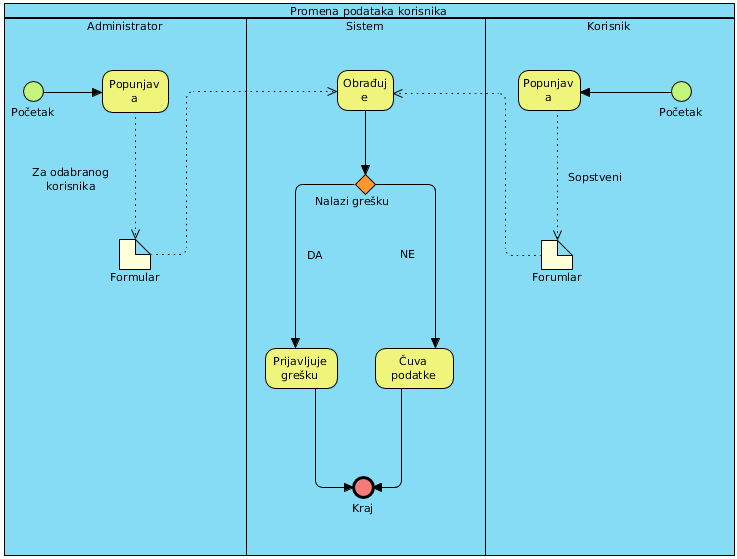
\includegraphics[width=0.9\linewidth]{PromenaPodatakaKorisnika.PNG}
    \caption{Promena podataka korisnika \cite{smalkov} \cite{vparadigm}}
    \label{fig:promenapodkor}
\end{figure}


\subsubsection{Promena korisničkih podataka}
\label{subsubsection:promenakorisnickihpodataka}
\begin{itemize}
    \item Akter: Administrator
    \item Kratak opis: Administrator sistema želi da promeni neke od ličnih podataka drugih korinika
    \item Preduslovi: Nema
    \item Postuslovi: Nema
    \item Osnovni tok događaja:
        \begin{enumerate}
            \item Administrator šalje sistemu zahtev za prikaz spiska korisnika kojima može menjati lične informacije.
            \item Sistem prikazuje administratoru sistema spisak korisika.
            \item Administrator bira željenog korisnika.
            \item Sistem prikazuje administrator formular na kome može menjati lične podatke korisnika (sve osim email-a).
            \item Administrator menja lične podatke koristika.
            \item Administrator šalje sistemu zahtev za čuvanje novih ličnih podataka korisnika.
            \item Sistem je uspešno promenio podatke odaranog korisnika.
            \item Sistem obaveštava administratora o uspešnoj akciji.
        \end{enumerate}
    \item Alternativni tok događaja:
        \begin{enumerate}
            \item Neko od obaveznih polja nije popunjeno ili neko od polja ne odgovara formatu koji je za to polje zadat regularnim izrazom
                \begin{enumerate}
                    \item U 7. koraku osnovnog toka sistem ispisuje poruku o grešci i obaveštava administratora da podaci nisu uspešno izmenjeni.
                    \item Administrator se vraća na 5. korak osnovnog toka.
                \end{enumerate}
        \end{enumerate}
\end{itemize}

\newpage

\subsection{Upravljanje izdanjem časopisa}
\label{subsection:upravljanjeizdanjemsec}

Kao što je prikazano na slici \ref{fig:upravljanjeizdanjem}, proces se sastoji od \textit{Odabira prihvaćenih radova za tekuće izdanje časopisa}, \textit{Pregleda radne verzije izdanja časopisa}, \textit{Pregled prethodnih izdanja časopisa}.
\begin{figure}[hbt!]
    \centering
    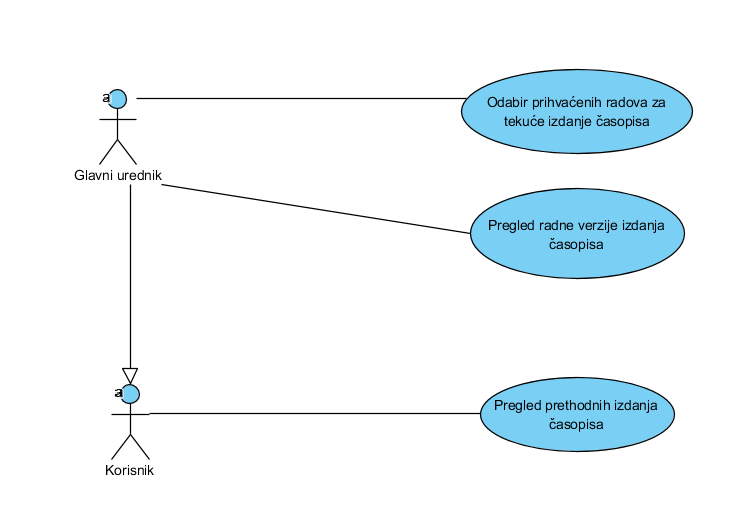
\includegraphics[width=\linewidth]{UpravljanjeIzdanjemCasopisa.PNG}
    \caption{Upravljanje izdanjem časopisa \cite{alex} \cite{vparadigm}}
    \label{fig:upravljanjeizdanjem}
\end{figure}

\subsubsection{Odabir prihvaćenih radova za tekuće izdanje časopisa}
\label{subsubsection:odabirradova}
\begin{itemize}
    \item Akter: Glavni urednik časopisa
    \item Kratak opis: Glavni urednik časopisa razmatra sve radove koji su prihvaćeni i vrši odabir radova koji će ući u tekuće izdanje časopisa.
    \item Preduslovi: Postoje prihvaćeni radovi koji nisu objavljeni
    \item Postuslovi: Nema
    \item Osnovni tok događaja:
        \begin{enumerate}
            \item Glavni urednik upućuje upit sistemu za sve prihvaćene radove koji nisu objavljeni ni u jednom dosadašnjem izdanju časopisa.
            \item Sistem vraća spisak svih takvih radova.
            \item Glavni urednik pregleda sledeći rad.
            \item Glavni urednik donosi odluku da li će rad ući u tekuće izdanje časopisa.
            \item Ukoliko će rad ući u tekuće izdanje: Glavni urednik šalje zahtev sistemu da se rad ubaci u radnu verziju tekućeg izdanja časopisa.
            \item Sistem dodaje rad u radnu verziju tekućeg izdanja.\\ Ponavljati korake 3, 4, 5 i 6 dok se postigne traženi broj radova ili traženi broj stranica za tekuće izdanje)
        \end{enumerate}
    \item Alternativni tok događaja:
        \begin{enumerate}
            \item Sistem ne vraća uspešno spisak prihvaćenih radova.
                \begin{enumerate}
                    \item U 2. koraku osnovnog toka, sistem ne vraća uspešno spisak prihvaćenih radova i obaveštava glavnog urednika o grešci.
                    \item Glavni urednik se vraća na 1. korak osnovnog toka ili se obraća se administratoru.
                \end{enumerate}
            \item Sistem ne otvara uspešno sledeći rad koji glavni urednik želi da pregleda.
                \begin{enumerate}
                    \item U 3. koraku osnovnog toka, sistem ne otvara uspešno rad koji glavni urednik želi da pregleda i prikazuje obaveštenje o grešci.
                    \item Glavni urednik se vraća na 3. korak osnovnog toka ili se obraća administratoru časopisa.
                \end{enumerate}
            \item Sistem ne dodaje rad u radnu verziju tekućeg izdanja.
            \begin{enumerate}
                \item Sistem ne dodaje rad u radnu verziju tekučeg izdanja i prikazuje poruku o grešci.
                \item Glavni urednik se vraća na 6. korak osnovnog toka ili se obraća administratoru.
            \end{enumerate}
        \end{enumerate}
\end{itemize}

\newpage

\subsubsection{Pregled radne verzije izdanja časopisa}
\label{subsubsection:pregledradneverzije}
\begin{itemize}
    \item Akter: Glavni urednik
    \item Kratak opis: Glavni urednik vrši pregled radne verzije tekućeg izdanja časopisa.
    \item Preduslovi: Nema
    \item Postuslovi: Nema
    \item Osnovni tok događaja:
        \begin{enumerate}
            \item Glavni urednik zahteva od sistema pregled radne verzije tekućeg izdanja časopisa.
            \item Sistem prikazuje radnu verziju tekućeg izdanja časopisa.
        \end{enumerate}
    \item Alternativni tok događaja:
        \begin{enumerate}
            \item Sistem ne prikazuje radnu verziju časopisa.
            \begin{enumerate}
                \item U 2. koraku osnovnog roka, sistem ne prikazuje radnu verziju časopisa i obaveštava glavnog urednika o grešci.
                \item Glavni urednik se vraća na 1. korak osnovnog toka ili se obraća administratoru.
            \end{enumerate}
        \end{enumerate}
        \begin{figure}[hbt!]
    \centering
    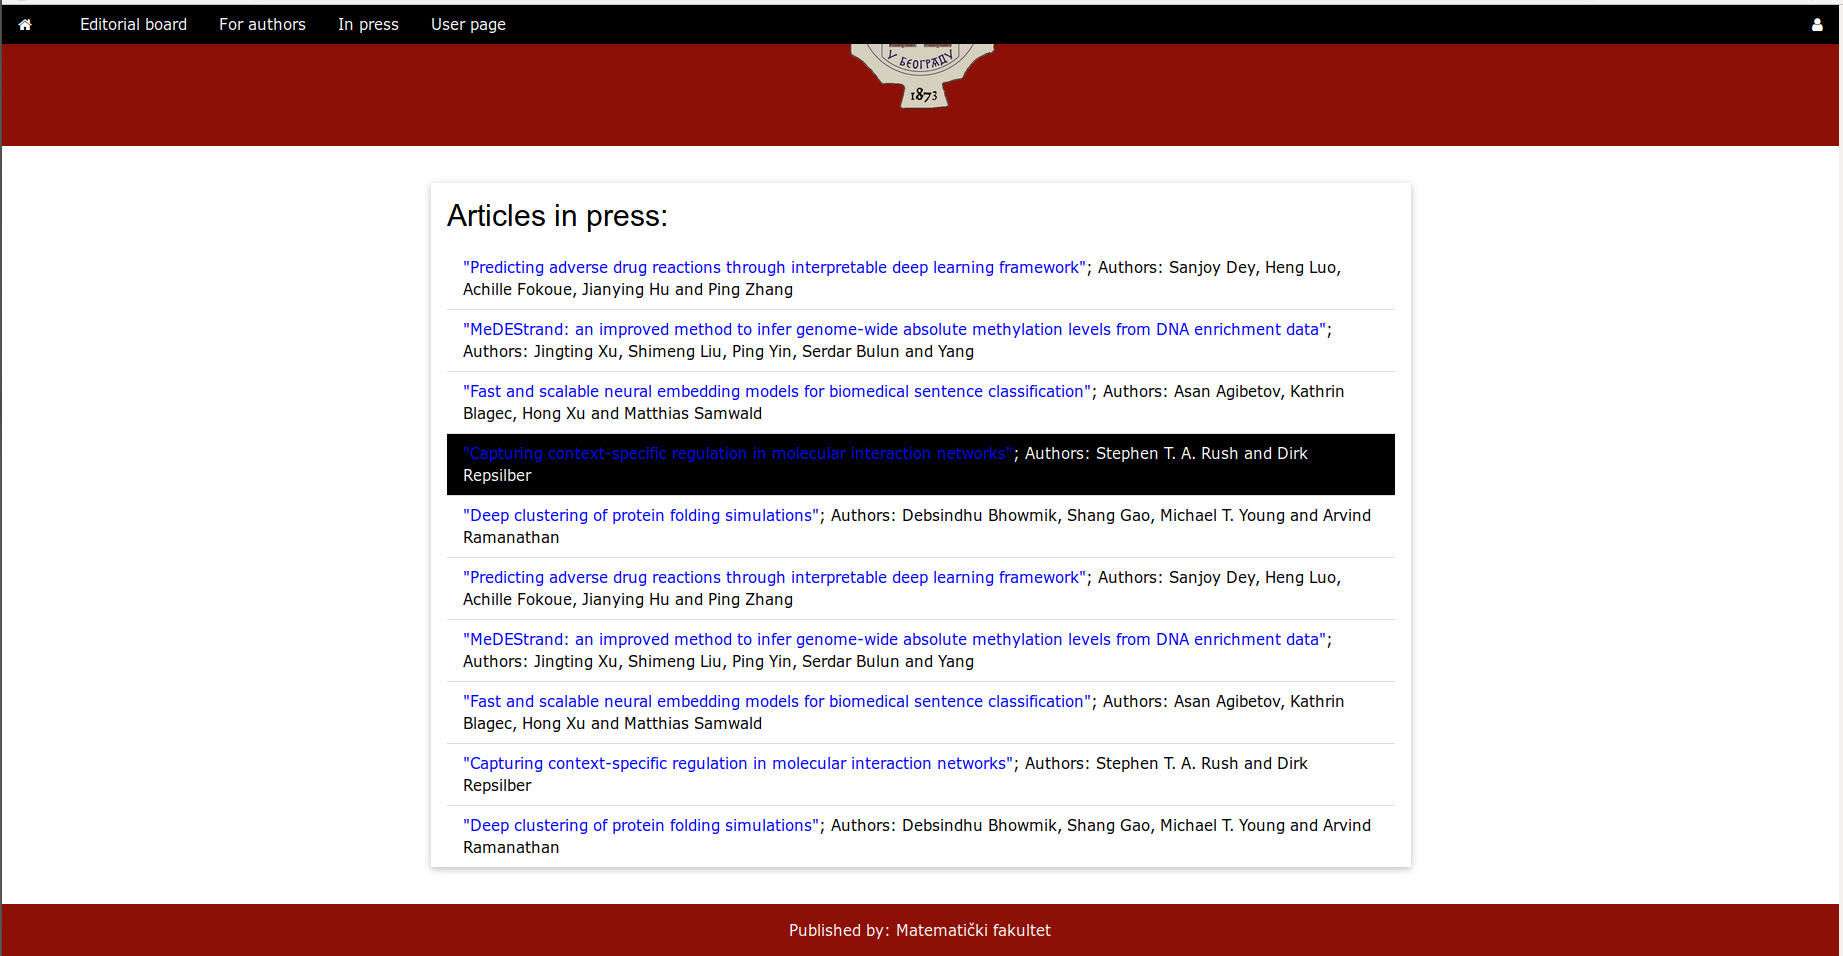
\includegraphics[width=\linewidth]{inpress.png}
    \caption{Pregled radne verzije izdanja časopisa \cite{vesnik}}
    \label{fig:inpress}
\end{figure}
\end{itemize}

\newpage

\subsubsection{Pregled prethodnih izdanja časopisa}
\begin{itemize}
    \item Akter: Korisnik
    \item Kratak opis: Korisnik informacionog sistema vrši pregled prethodnog izdanja časopisa.
    \item Preduslovi: Postoji bar jedno izdanje časopisa.
    \item Postuslovi: Nema
    \item Osnovni tok događaja:
        \begin{enumerate}
            \item Korisnik zahteva od sistema pregled spisak prethodnih izdanja časopisa.
            \item Sistem prikazuje spisak prethodnih izdanja.
            \item Korisnik bira izdanje koje želi da pregleda.
            \item Sistem mu prikazuje traženo izdanje časopisa.
        \end{enumerate}
    \item Alternativni tok događaja:
        \begin{enumerate}
            \item Sistem ne prikazuje spisak prethodnih izdanja.
            \begin{enumerate}
                \item Sistem ne prikazuje spisak prethodnih izdanja časopisa i obaveštava korisnika o grešci.
                \item Korisnik se vraća na 1. korak osnovnog toka, odustaje ili se obraća administratoru.
            \end{enumerate}
            \item Sistem ne prikazuje traženo izdanje časopisa.
            \begin{enumerate}
                \item Sistem ne prikazuje traženo izdanje časopisa i obaveštava korisnika o grešci.
                \item Korisnik se vraća na 3. korak osnovnog toka, pri čemu eventualno menja izdanje koje želi da pregleda, ili se obraća administratoru.
            \end{enumerate}
        \end{enumerate}
\end{itemize}

\newpage

\subsection{Upravljanje časopisom}
\label{subsection:upravljanjecasopisom}

\subsubsection{Promena podataka časopisa}
\label{subsection:promenapodatakacasopisasec}

\begin{figure}[hbt!]
    \centering
    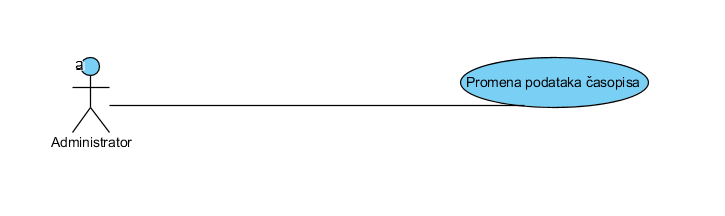
\includegraphics[width=\linewidth]{PromenaPodatakaCasopisa.png}
    \caption{Promena podataka časopisa \cite{alex} \cite{vparadigm}}
    \label{fig:promenapodcas}
\end{figure}

\begin{itemize}
    \item Akter: Administrator sistema
    \item Kratak opis: Administrator menja podatke časopisa
    \item Preduslov: nema
    \item Postuslov: nema
    \item Osnovni tok događaja:
        \begin{enumerate}
            \item Administrator pristupa obrascu za menjanje podataka
            \item Administrator unosi podatke u formu
            \item Adminstrator šalje zahtev za čuvanjem novih podataka
            \item Sistem je sačuvao nove podatke
            \item Sistem obaveštava koriniska o sačuvanim izmenama
        \end{enumerate}
    \item Alternativni tok događaja:
        \begin{enumerate}
            \item Koraka 4. osnovnog toka: Sistem ne može da sačuva nove podatke
                \begin{enumerate}
                    \item Administrator popravlja unete podatke tako da budu u saglasnosti sa bazom podataka
                    \begin{enumerate}
                        \item Administrator šalje zahtev za čuvanjem podataka
                        \item Ako je sistem sačuvao nove podatke, prelazi se na korak 5. osnovnog toka.
                        \item Ako ne, prelazi se na korak 1.b) alternativnog toka.
                    \end{enumerate}
                    \item Administrator proverava internet konekciju i uspešno je podešava.
                    \begin{enumerate}
                        \item Ponovo šalje zahtev za čuvanjem podataka
                        \item Ako je sistem sačuvao nove podatke, prelazi se na korak 5. osnovnog toka.
                        \item Ako ne, prelazi se na korak 1.c) alternativnog toka.
                    \end{enumerate}
                    \item Administrator proverava da li je funkcionalnost slanja podataka preko forme dobro implementirana.
                    \begin{enumerate}
                        \item Administrator popravlja funkcionalnost i pokušava ponovo da sačuva podatke.
                        \item Administrator šalje zahtev za čuvanjem podataka
                        \item Ako je sistem sačuvao nove podatke, prelazi se na korak 5. osnovnog toka.
                        \item Ako ne, prelazi se na korak 1.d) alternativnog toka.
                    \end{enumerate}
                    \item Ozbiljna greška sistema. Administrator traži grešku i pokušava da je otkloni.
                \end{enumerate}
        \end{enumerate}
        \item Dodatak: slika \ref{fig:promenapodatkacasopisa}
        \begin{figure}[hbt!]
    \centering
    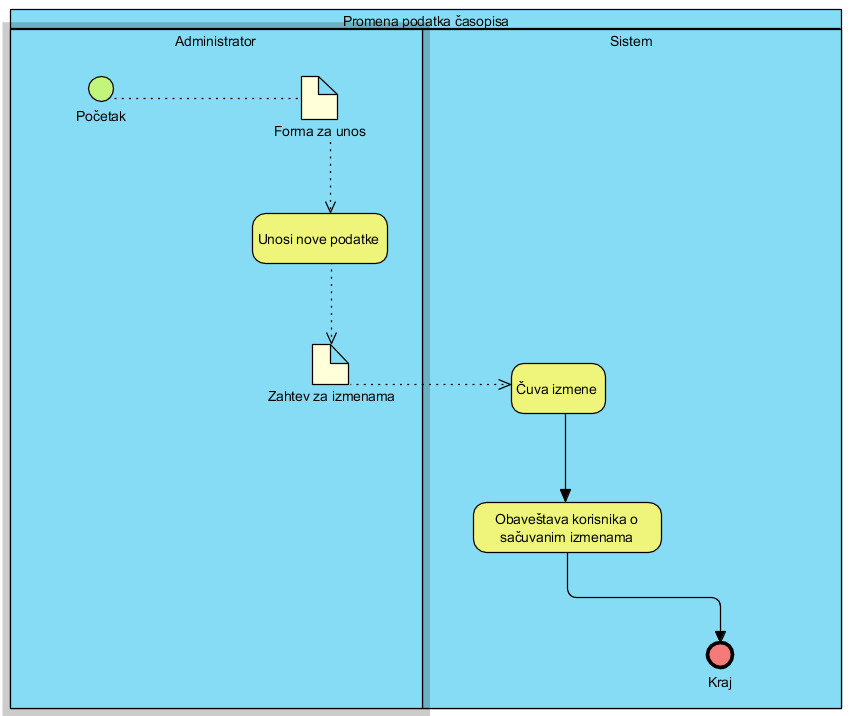
\includegraphics[width=\linewidth]{PromenaPodatakaCasopisa.PNG}
    \caption{Promena podataka časopisa \cite{smalkov} \cite{vparadigm}}
    \label{fig:promenapodatkacasopisa}
\end{figure}
\end{itemize} 
\newpage

\subsection{Upravljanje radovima}
\label{subsection:upravljanjeradovimasec}

Kao što je prikazano na slikama \ref{fig:nivo1} i \ref{fig:upravljanjeradovima}, proces se sastoji od: \textit{prijavljivanje radova}, \textit{Ažuiriranje radova}, \textit{Povlačenje rada}, \textit{Odlučivanje o statusu rada}, \textit{Komentarisanje rada}
\begin{figure}[hbt!]
    \center
    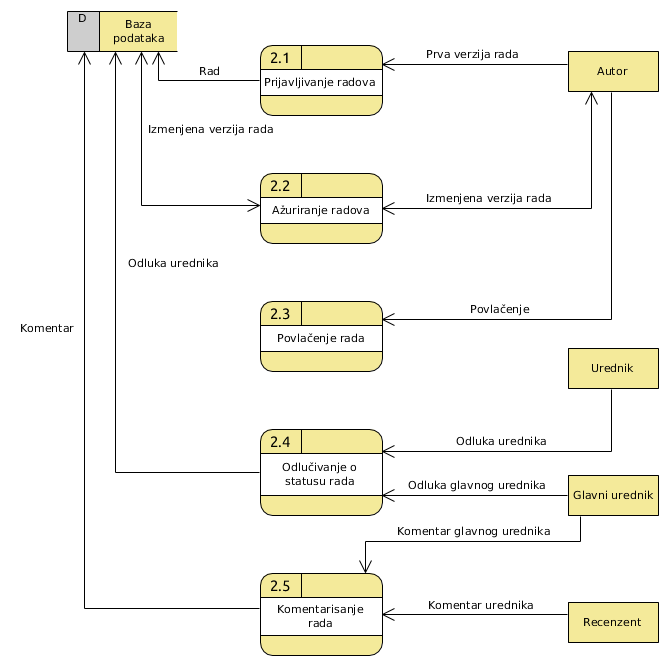
\includegraphics[width=1.05\linewidth]{UpravljanjeRadovima1.png}
    \caption{Dijagram toka podataka nivoa 1; Upravljanje radovima \cite{smalkov} \cite{vparadigm}}
    \label{fig:nivo1}
\end{figure}
\begin{figure}[hbt!]
    \centering
    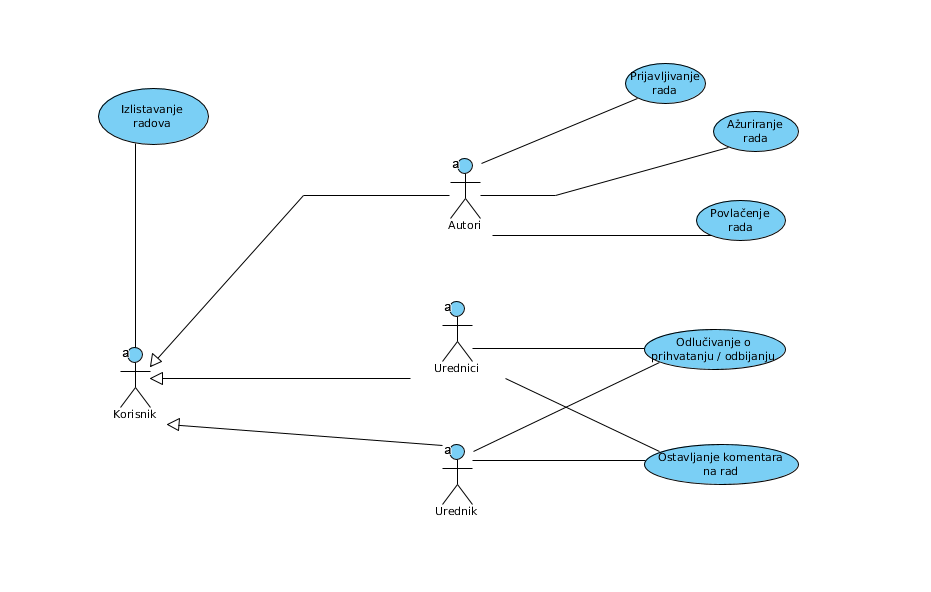
\includegraphics[width=1.05\linewidth]{UpravljanjeRadovima.png}
    \caption{Upravljanje radovima \cite{alex} \cite{vparadigm}}
    \label{fig:upravljanjeradovima}
\end{figure}

\subsubsection{Izlistavanje radova}
\label{subsubsection:izlistavanjeradova}
\begin{itemize}
    \item Akter: Korisnik
    \item Kratak opis: Korisnik izlistava radove po zadatom uslovu u filteru.
    \item Preduslovi: Korisnik je registrovan u sistemu.
    \item Postuslovi: Nema
    \item Osnovni tok događaja:
        \begin{enumerate}
            \item Korisnik bira kriterijum u filteru.
            \item Korisnik šalje zahtev sistemu za prikazivanje svih radova koji zadovoljavaju zadati kriterijum.
            \item Sistem šalje podatke o radovima i islistava ih.
        \end{enumerate}
    \item Alternativni tok događaja:
        \begin{enumerate}
            \item Korak 2. osnovnog toka: Sistem ne nalazi podatke ni o jednom radu.
            \begin{enumerate}
                \item Sistem obaveštava korisnika o nepostojanju radova sa zadatim kriterijumom.
                \item Korisnik se vraća na 1. korak osnovnog toka ili odustaje.
            \end{enumerate}
        \end{enumerate}
\end{itemize}

\newpage

\begin{comment}
\subsubsection{Recenzent izlistava radove koje recenzira}
\begin{itemize}
    \item Akter: Recenzent
    \item Kratak opis: Recenzent izlistava radove na koje je prihvatio da recenzira.
    \item Preduslovi: Recenzent je korisnik sistema sa ulogom Recenzent.
    \item Postuslovi: Nema
    \item Osnovni tok događaja:
        \begin{enumerate}
            \item Recenzent šalje zahtev sistemu za prikazivanje svih radova koje je prihvatio da recenzira.
            \item Sistem šalje podatke o radovima i islistava ih.
        \end{enumerate}
    \item Alternativni tok događaja:
        \begin{enumerate}
            \item Korak 2. osnovnog toka: Sistem ne nalazi podatke ni o jednom radu.
            \begin{enumerate}
                \item Sistem obaveštava korisnika o nepostojanju radova na kojima je prihvatio recenzentsku ulogu.
                \item Recenzent se vraća na 1. korak osnovnog toka ili odustaje.
            \end{enumerate}
        \end{enumerate}
\end{itemize}

\subsubsection{Urednik izlistava radove}
\begin{itemize}
    \item Akter: Urednik
    \item Kratak opis: Urednik izlistava radove koje je dobio od glavnog uredinka.
    \item Preduslovi: Recenzent je korisnik sistema sa ulogom Recenzent.
    \item Postuslovi: Nema
    \item Osnovni tok događaja:
        \begin{enumerate}
            \item Recenzent šalje zahtev sistemu za prikazivanje svih radova koje je prihvatio da recenzira.
            \item Sistem šalje podatke o radovima i islistava ih.
        \end{enumerate}
    \item Alternativni tok događaja:
        \begin{enumerate}
            \item Korak 2. osnovnog toka: Sistem ne nalazi podatke ni o jednom radu.
            \begin{enumerate}
                \item Sistem obaveštava korisnika o nepostojanju radova na kojima je prihvatio recenzentsku ulogu.
                \item Recenzent se vraća na 1. korak osnovnog toka ili odustaje.
            \end{enumerate}
        \end{enumerate}
\end{itemize}
\end{comment}

\subsubsection{Prijavlivanje rada}
\label{subsubsection:prijavljivanjerada}

\begin{itemize}
    \item Akter: Autor
    \item Kratak opis: Autor prijavljuje rad.
    \item Preduslovi: Autor je korisnik sistema sa ulogom Autor.
    \item Postuslovi: Rad se nalazi u sistemu.
    \item Osnovni tok događaja:
        \begin{enumerate}
            \item Autor unosi potrebne podatke podatke za rad.
            \item Autor šalje zahtev za prijavljivanje rada.
            \item Sistem čuva rad.
            \item Sistem obaveštava autora o uspešnom prijavljivanju rada.
        \end{enumerate}
    \item Alternativni tok događaja:
        \begin{enumerate}
            \item Korak 3. osnovnog toka: Sistem nije uspeo da sačuva rad.
            \begin{enumerate}
                \item Sistem obaveštava korisnika o grešci.
                \item Autor se vraća na 1. korak osnovnog toka ili odustaje.
            \end{enumerate}
        \end{enumerate}
    \item Dodatak: slika \ref{fig:prijavljivanje}
    \begin{figure}[hbt!]
    \centering
    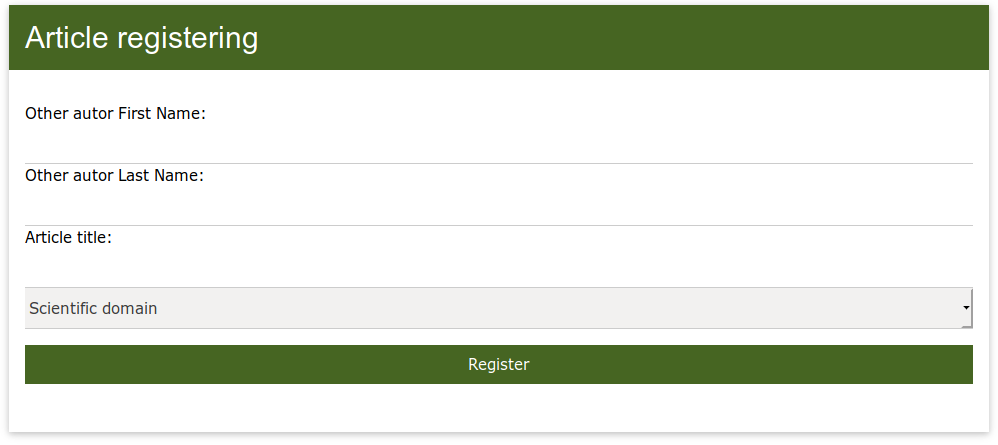
\includegraphics[width=1\linewidth]{ArticleRegister.png}
    \caption{Prijavljivanje rada}
    \label{fig:prijavljivanje}
\end{figure}
\end{itemize}

\newpage

\subsubsection{Ažuriranje rada}
\label{subsubsection:azuriranje}
\begin{itemize}
    \item Akter: Autor
    \item Kratak opis: Autor, nakon dorade, prijavljuje novu verziju rada
    \item Preduslovi: Rad je prijavljen
    \item Postuslovi: Nova verzija rada je sačuvana
    \item Osnovni tok događaja:
        \begin{enumerate}
           \item Autor popunjava formular za prijavu nove verzije rada.
           \item Autor šalje zahtev za čuvanjem nove verzije rada.
           \item Sistem je sačuvao novu verziju rada.
           \item Sistem obaveštava autora o sačuvanoj novoj verziji rada.
        \end{enumerate}
    \item Alternativni tok događaja:
        \begin{enumerate}
            \item Korak 3. osnovnog toka: Sistem nije uspeo da sačuva novu verziju rada.
            \begin{enumerate}
                \item Sistem obaveštava korisnika o grešci.
                \item Autor se vraća na 1. korak osnovnog toka ili odustaje.
            \end{enumerate}
        \end{enumerate}
\end{itemize}

\newpage

\subsubsection{Povlačenje rada}
\label{subsubsection:povlacenjerada}
\begin{itemize}
    \item Akter: Autor
    \item Kratak opis: Autor povlači rad iz časopisa
    \item Preduslovi: Rad je prijavljen
    \item Postuslovi: Nema
    \item Osnovni tok događaja:
        \begin{enumerate}
           \item Autor popunjava formular za povlačenjem rada.
           \item Autor šalje zahtev za povlačenjem rada.
           \item Sistem je označio rad kao povučen, ali ga nije izbrisao iz baze podataka.
           \item Sistem obaveštava autora da je rad povučen.
        \end{enumerate}
    \item Alternativni tok događaja: nema
\end{itemize}

\newpage

\subsubsection{Odlučivanje o prihvatanju/odbijanju rada}
\label{subsubsection:prihvatanjeodbijanje}
\begin{itemize}
    \item Akter: Glavni urednik, Urednik
    \item Kratak opis: (Glavni) Urednik menja prihvata ili odbija rad. Glavni urednik može promeniti ovaj status već prihvaćenom/odbijenom radu.
    \item Preduslovi: Rad se nalazi u sistemu. Uredniku je rad prosledjen od strane glavnog urednika. Uradnik i Glavni urednik su registrovani u sistemu
    \item Postuslovi: Rad ima novo stanje u sistemu.
    \item Osnovni tok događaja:
        \begin{enumerate}
            \item (Glavni) Urednik odabira rad.
            \item (Glavni) Urednik bira da li je rad odbijen ili prihvaćen.
            \item (Glavni) Urednik šalje sistemu zahtev za čuvanjem novog statusa rada.
            \item Sistem je sačuvao novi status rada.
            \item Sistem obaveštava (glavnog) urednika o uspešnom prihvatanju/odbijanju rada.
        \end{enumerate}
    \item Alternativni tok događaja:
        \begin{enumerate}
            \item Korak 2. osnovnog toka: Rad prethodno nije recenziran.
                \begin{enumerate}
                    \item (Glavnom) Uredniku se prikazuje polje u kom ostavlja komentar na rad.
                    \item (Glavni) Urednik se vraća na 3. korak osnovnog toka ili odustaje.
                \end{enumerate}
            \item Korak 4. osnovnog toka: Sistem nije uspeo da sačuva rad.
            \begin{enumerate}
                \item Sistem obaveštava (glavnog) urednika o grešci.
                \item (Glavni) Urednik se vraća na 1. korak osnovnog toka ili odustaje.
            \end{enumerate}
        \end{enumerate}
\end{itemize}

\newpage

\subsubsection{Ostavljanje komentara na rad}
\label{subsubsection:ostavljanjekomentara}
\begin{itemize}
    \item Akter: Glavni urednik i urednik
    \item Kratak opis: Glavni urednik i urednik ostavljaju komentar na rad
    \item Preduslovi: Rad je prijavljen
    \item Postuslovi: Komentar je sačuvan
    \item Osnovni tok događaja:
        \begin{enumerate}
           \item (Glavni) urednik bira rad na koji želi da ostavi komentar.
           \item (Glavni) urednik piše tekst komentara.
           \item (Glavni) urednik šalje zahtev za čuvanjem komentara.
           \item Sistem je sačuvao komentar.
           \item Sistem šalje poruku sa odgovarajućim šablonom autoru koji je prijavio rad. 
           \item Sistem obaveštava (glavnog) urednika o ostavljanju komentara na rad.
        \end{enumerate}
    \item Alternativni tok događaja:
        \begin{enumerate}
            \item Koraka 2. osnovnog toka: (Glavni) urednik nije ukucao nikakav tekst
            \begin{enumerate}
                \item Sistem ignoriše zahtev.
                \item Sistem obaveštava (glavnog) urednika o tome da nije uneo tekst.
                \item Tok se nastavlja na koraku 1 glavnog toka.
            \end{enumerate}
            \item Korak 5. osnovnog toka: Sistem nije uspeo da pošalje poruku autoru.
            \begin{enumerate}
                \item Sistem obaveštava (glavnog) urednika da nije poslao poruku autoru o novom komentaru na rad.
                \item Sistem obaveštava (glavnog) urednika da je potrebno da sam obavesti autora o novom komentaru.
                \item Tok se nastavlja na koraku 6 glavnog toka.
            \end{enumerate}
        \end{enumerate}
        \item Dodatak: slika \ref{fig:leavingcomment}
        \begin{figure}[ht!]
    \centering
    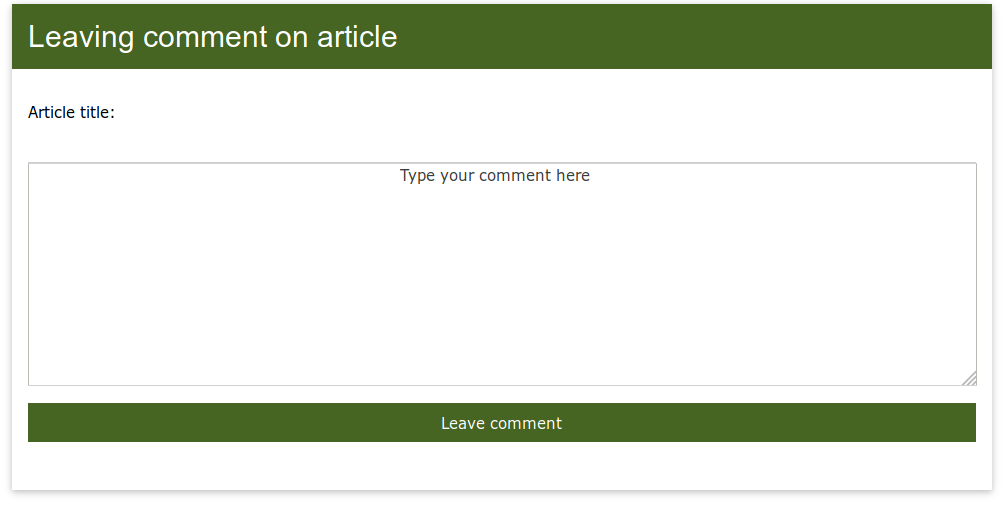
\includegraphics[width=0.8\linewidth]{LeavingComment.png}
    \caption{Ostavljanje komentara na rad}
    \label{fig:leavingcomment}
\end{figure}
\end{itemize}

\vspace{1.5cm}

\newpage

\subsection{Recenziranje}
\label{subsection:recenziranjesec}

\begin{figure}[ht!]
    \centering
    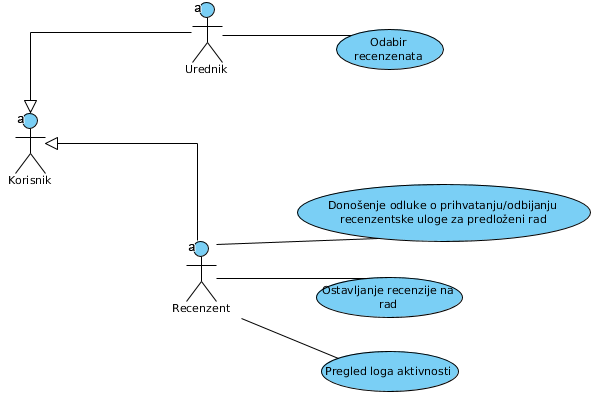
\includegraphics[width=\linewidth]{RecenziranjeUseCase.PNG}
    \caption{Dijagram slučaja upotrebe Recenziranje \cite{alex} \cite{vparadigm}}
    \label{fig:recenziranjeusecase}
\end{figure}

\subsubsection{Odabir recenzenta}
\label{subsubsection:odabirrecenzenta}
\begin{itemize}
    \item Akter: Urednik
    \item Kratak opis: Urednik bira recenzente za prijavljeni rad
    \item Preduslovi: Nema
    \item Postuslovi: Nema
    \item Osnovni tok događaja:
        \begin{enumerate}
           \item Urednik šalje sistemu zahtev za dobijanje spiska recenzenata.
           \item Sistem prikazuje spisak recenzenata.
           \item Urednik bira recenzenta.
           \item Urednik šalje recenzentu ponudu za recenziranje rada.
           \item Sistem šalje mejl recenzentu sa ponudom za recenziranje.
           \item Sistem obaveštava urednika o uspešno poslatom mejlu. 
           \item Sistem u bazi podataka dodeljuje radu odabranog recenzenta
        \end{enumerate}
    \item Alternativni tok događaja:
        \begin{enumerate}
            \item Sistem ne prikazuje spisak recenzenata zbog greške.
            \begin{enumerate}
                \item U 2. koraku osnovnog toka, sistem ne prikazuje spisak recenzenata i prikazuje poruku o grešci.
                \item Urednik se vraća na 1. korak osnovnog toka ili se obraća administratoru.
            \end{enumerate}
            \item Nema recenzenata u sistemu.
            \begin{enumerate}
                \item U 2. koraku osnovnog toka, sistem prikazuje prazan spisak recenzenata.
                \item Urednik se obraća glavnom uredniku.
            \end{enumerate}
            \item Sistem nije uspešno poslao mejl recenzentu.
            \begin{enumerate}
                \item U 5. koraku osnovnog toka, sistem nije uspešno poslao mejl recenzentu,
                \item Urednik se vraća na 4. korak osnovnog toka ili se obraća administratoru.
            \end{enumerate}
        \end{enumerate}
        \item Dodatak: slika \ref{fig:recenziranje}
        \afterpage{\clearpage}
        \begin{sidewaysfigure}[ht!]
    \centering
    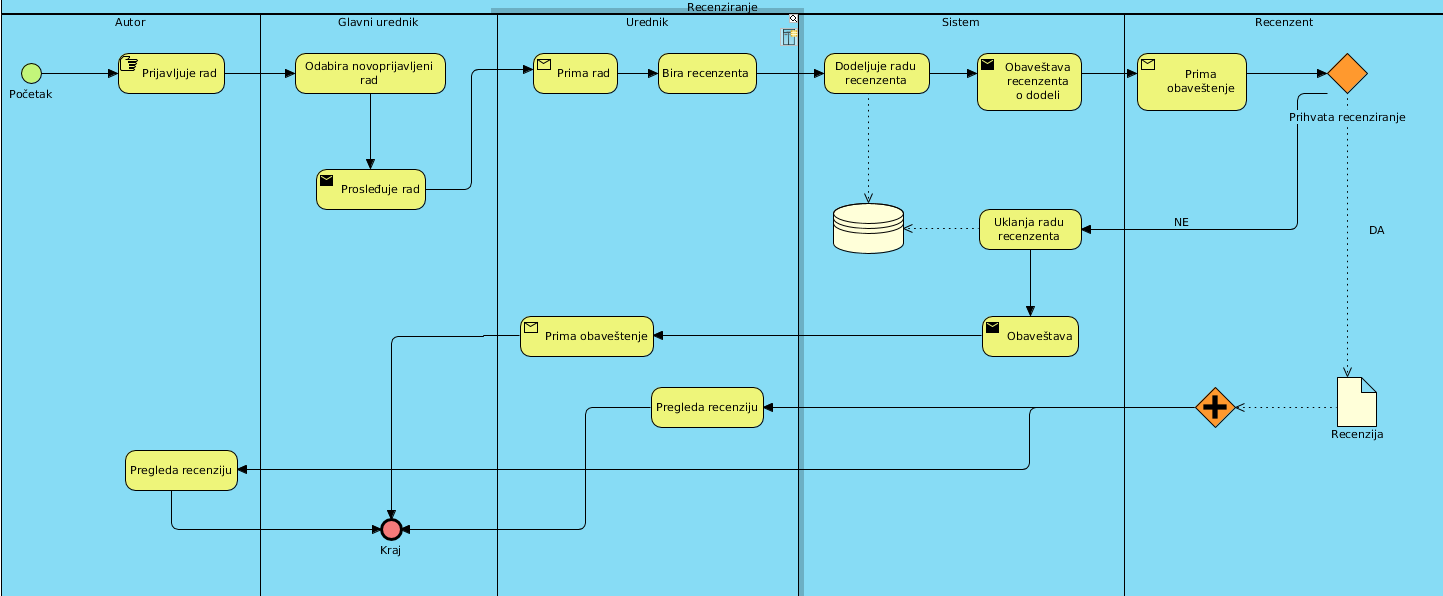
\includegraphics[width=1\linewidth]{Recenziranje.PNG}
    \caption{Recenziranje \cite{smalkov} \cite{vparadigm}}
    \label{fig:recenziranje}
\end{sidewaysfigure}
\end{itemize}

\newpage

\subsubsection{Donošenje odluke o prihvatanju/odbijanju recenzentske uloge}
\label{subsubsection:prihvatanjeodbijanjeuloge}
\begin{itemize}
    \item Akter: Recenzent
    \item Kratak opis: Recenzent donosi odluku da li prihvata ili odbija recenzentsku ulogu za prijavljeni rad.
    \item Preduslovi: Recenzent je dobio ponudu da recenzira rad.
    \item Postuslovi: Nema
    \item Osnovni tok događaja:
        \begin{enumerate}
            %\item Recenzent donosi odluku da li prihvata da recenzira rad.
            %\item Recenzent prihvata da recenzira rad.
            %    \begin{enumerate}
            %        \item Slučaj upotrebe se završava.
            %    \end{enumerate}
            \item Recenzent odbija da recenzira rad.
                \begin{enumerate}
                    \item Recenzent šalje zahtev sistemu za uklanjanje sa spiska recenzenata za taj rad.
                    \item Sistem otvara formular za pisanje mejla uredniku.
                    \item Recenzent šalje odgovor uredniku.
                    \item Sistem šalje mejl uredniku.
                    \item Sistem uklanja recenzenta sa spiska.
                    \item Sistem obaveštava recenzenta o uspešnom uklanjanju sa spiska.
                \end{enumerate}
        \end{enumerate}
    \item Alternativni tok događaja:
        \begin{enumerate}
            \item Sistem ne šalje mejl uredniku.
            \begin{enumerate}
                \item U koraku (d) osnovnog toka sistem ne uklanja uspešno recenzenta sa spiska recenzenata za taj rad.
                \item Sistem obaveštava recenzenta o grešci.
                \item Recenzent se vraća na korak (d) osnovnog toka ili se obraća administratoru.
            \end{enumerate}
            \item Sistem ne uklanja recenzenta sa spiska.
            \begin{enumerate}
                \item U koraku (e) osnovnog toka sistem ne uklanja uspešno recenzenta sa spiska recenzenata za taj rad.
                \item Sistem obaveštava recenzenta o grešci.
                \item Recenzent se vraća na korak (a) osnovnog toka ili se obraća administratoru.
            \end{enumerate}
        \end{enumerate}
\end{itemize}

\newpage

\subsubsection{Ostavljanje recenzije na rad}
\label{subsubsection:ostavljanjerecenzijesec}
\begin{itemize}
    \item Akter: Recenzent
    \item Kratak opis: Recenzent ostavlja svoju recenziju na rad u sistemu.
    \item Preduslov: Recenzent je dodeljen datom radu.
    \item Postuslov: Nema
    \item Osnovni tok događaja:
        \begin{enumerate}
            \item Recenzent popunjava polja formulara za recenziju.
            \item Recenzent šalje zahtev sistemu za objavljivanje recenzije.
            \item Sistem čuva podatke o receziji.
            \item Sistem obaveštava recenzenta o uspešno sačuvanoj recenziji.
        \end{enumerate}
    \item Alternativni tokovi:
        \begin{enumerate}
            \item Sistem ne čuva podatke o recenziji.
            \begin{enumerate}
                \item U 3. koraku osnovnog toka sistem ne čuva uspešno podatke o recenziji.
                \item Sistem obaveštava recenzenta o grešci.
                \item Recenzent se vraća na 2. korak osnovnog toka ili se obraća administratoru.
            \end{enumerate}
        \end{enumerate}
        \item Dodatak: slika \ref{fig:ostavljanjerecenzije}
        \begin{figure}[hbt!]
    \centering
    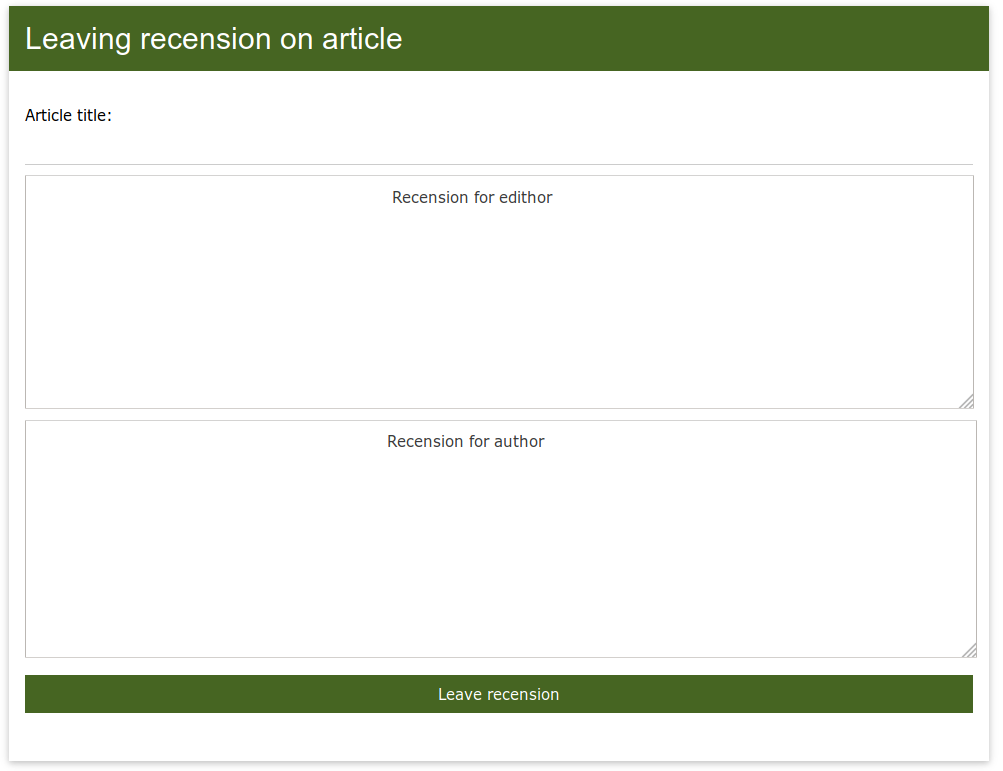
\includegraphics[width=0.7\linewidth]{LeavingRecension.png}
    \caption{Ostavljanje recenzije}
    \label{fig:ostavljanjerecenzije}
\end{figure}
\end{itemize}

\newpage

\subsubsection{Pregled loga aktivnosti}
\label{subsubsection:pregledloga}
\begin{itemize}
    \item Akter: Recenzent
    \item Kratak opis: Recenzent pregleda spisak svih radova koje je prihvatio ili odbio da recenzira
    \item Preduslov: Recenzent poseduje spisak aktivnosti
    \item Postuslov: Nema
    \item Osnovni tok događaja:
        \begin{enumerate}
            \item Recenzent zahteva spisak svojih aktivnosti
            \item Sistem ispisuje spisak aktivnosti
        \end{enumerate}
\end{itemize}

\newpage

\subsection{Komunikacija među korisnicima}
\label{subsection:komunikacijasec}
\begin{figure}[hbt!]
    \centering
    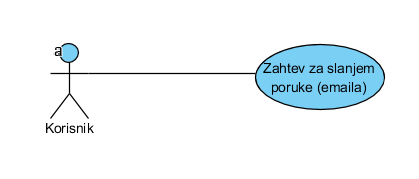
\includegraphics[width=0.5\linewidth]{KomunikacijaIzmedjuKorisnika.PNG}
    \caption{Komunikacija među korisnicima \cite{alex} \cite{vparadigm}}
    \label{fig:komunikacija}
\end{figure}

\subsubsection{Zahtev za slanje poruke (emaila)}
\begin{itemize}
    \item Akter: Korisnik
    \item Kratak opis: Korisnik šalje email koristeći usluge sistema
    \item Preduslovi: Korisnik je registrovan u sistemu.
    \item Postuslovi: Nema
    \item Osnovni tok događaja:
        \begin{enumerate}
            \item Korisnik zahteva spisak postojećih šablona.
            \item Sistem prikazuje korisniku spisak šablona.
            \item Korisnik bira željeni šablon.
            \item Sistem prikazuje sadržaj šablona.
            \item Korisnik označava da želi da nastavi sa slanjem šablona.
            \item Sistem prikazuje imena korisnika sistema.
            \item Korisnik bira korisnike sa liste.
            \item Korisnik šalje zahtev za slanjem poruke.
            \item Sistem šalje email na adresu korisnika.
            \item Sistem obaveštava korisnika o uspešno poslatoj poruci.
        \end{enumerate}
    \item Alternativni tok događaja:
        \begin{enumerate}
            \item Korak 5. osnovnog toka: Korisnik želi da izmeni šablon.
            \begin{enumerate}
                \item Korisnik vrši potrebne izmene u tekstu ili izmenu šablona.
                \item Ako korisnik ne želi da se novi šablon sačuva u bazi prelazi na korak 5 glavnog toka.
                \item Korisnik šalje sistemu zahtev za čuvanjem novog šablona.
                \item Sistem čuva šablon.
                \item Sistem obaveštava korisnika o čuvanju šablona.
                \item Korisnik se vraća na 5. korak osnovnog toka.
            \end{enumerate}
        \end{enumerate}
    \item Dodatak: spisak šablona i njihov izgled na slici \ref{fig:template} i opis toka slanja na slici \ref{fig:tok}
    \begin{figure}[h!]
    \centering
    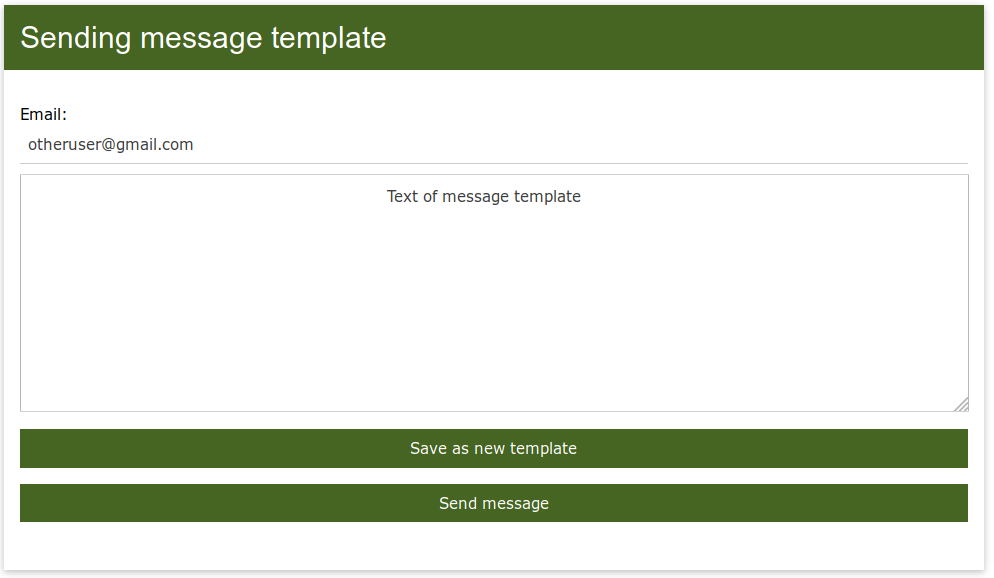
\includegraphics[width=1\linewidth]{SendingTemplate.png}
    \caption{Izgled šablona}
    \label{fig:template}
    \end{figure}
    \begin{figure}[h!]
    \centering
    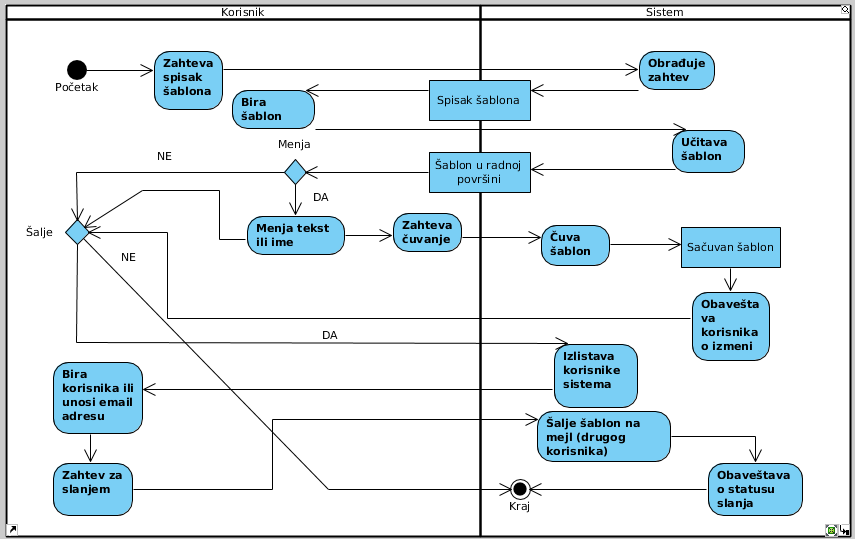
\includegraphics[width=1.05\linewidth]{KomunikacijaMedjuKorisnicima.PNG}
    \caption{Tok slanja \cite{alex} \cite{vparadigm}}
    \label{fig:tok}
    \end{figure}
    \begin{itemize}
        \item Glavni urednik urednicima: obaveštava urednika o novopristriglom radu i prosleđuje mu rad
        \item Glavni urednik administratoru: obaveštava administratora da želi da ukloni korisnika iz sistema
        \item Urednik autoru: obaveštava autora o tome da li je rad prihvaćen ili odbijen 
        \item Recenzent uredniku: obaveštava ga da ne želi da prihvati recenziju na predloženi rad
        \item Sistem autoru: obaveštava ga kada (glavni) urednik ostavi komentar na rad, ili kada recenzent ostavi recenziju
    \end{itemize}
\end{itemize}

\newpage

\section{Model baze podataka}
\label{section:modelbaze}

Dijagrami koji opisuju bazu podataka nalaze se na slikama \ref{fig:er} i \ref{fig:eer}, pri čemu dole navedeni tekst opisuje drugu.
\begin{figure}[hbt!]
    \centering
    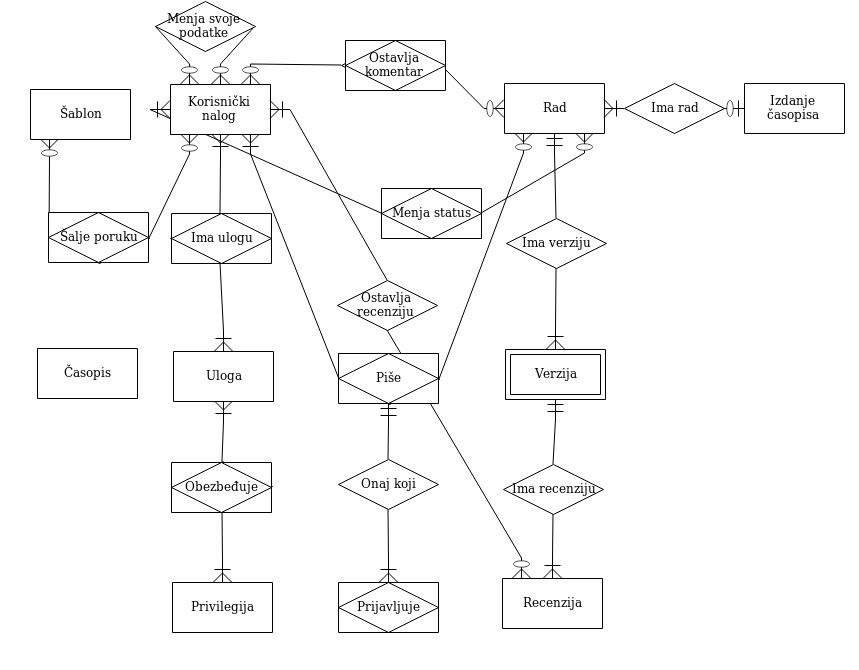
\includegraphics[width=1.15\linewidth]{ERDiagram.png}
    \caption{ER dijagram \cite{erdplus}}
    \label{fig:er}
\end{figure}
\afterpage{\clearpage}
\begin{sidewaysfigure}[ht!]
    \centering
    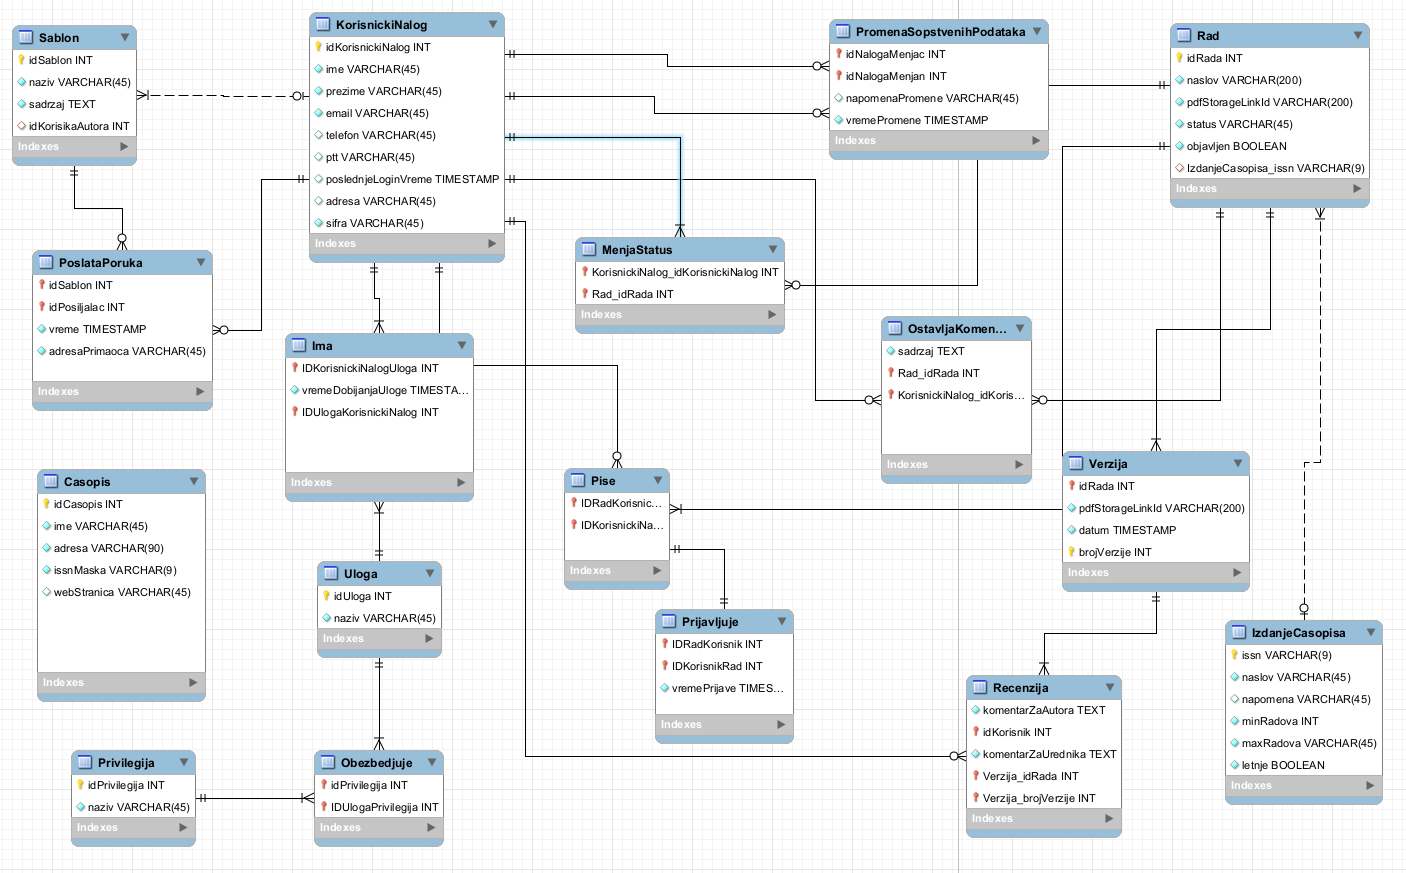
\includegraphics[width=1.15\linewidth]{EER.png}
    \caption{EER dijagram \cite{wbench}}
    \label{fig:eer}
\end{sidewaysfigure}

\begin{itemize}
    \item Nezavisni entiteti
    \begin{itemize}
        \item Korisnički nalog
        \item Uloga
        \item Privilegija
        \item Šablon
        \item Rad
        \item Recenzija
        \item Časopis
        \item Izdanje časopisa
    \end{itemize}
    \item Agregirani entiteti
    \begin{itemize}
        \item Ima
        \item Piše
        \item Obezbeđuje
        \item Prijavljuje
        \item Ostavlja komentar
        \item Poslata poruka
    \end{itemize}
    \item Rekurzivni odnos
    \begin{itemize}
        \item Promena sopstvenih podataka
    \end{itemize}
    \item Slab entitet ili odnos specijalizacija/generalizacija
    \begin{itemize}
        \item Zavisni entitet: Verzija
    \end{itemize}
    \item Trigeri kojima se menja stanje baze
    \begin{itemize}
        \item Triger1 - Prilikom pravljenja nove verzije rada, link rada se postavlja na link verzije
        \item Triger2 - Prilikom pravljenja nove verzije rada se automatski postavljaju datum i vreme na trenutan datum i vreme
        \item Triger3 - Prilikom prijave rada se automatski pravi i njegova prva verzija
        \item Prilikom prijave novog korisnika automatski mu se dodeljuje i status autora
    \end{itemize}
\end{itemize}

\newpage

\section{Arhitektura}
\label{section:arhitekturasec}
    
    Karakteristike arhitekture informacionog sistema:
    \begin{itemize}
        \item Tip aplikacije: Web aplikacija. Ovakav odabir sistemu obezbeđuje \textit{dostupnost}, \textit{ažurnost} i \textit{jednostavnost}.
        \item Strategije isporučivanja: jedan serverski i više klijentskih računara
        \item Odgovarajuće tehnologije: HTML, CSS, SQL, JavaScript(jQuery, Angular.js/React.js),\\
        PHP(Simphony)/Java(Spring MVC)
    \end{itemize}
    
    \subsection{Tip arhitekture:}
    \label{sbsection:tip}
    
     \begin{figure}[hbt!]
    \centering
    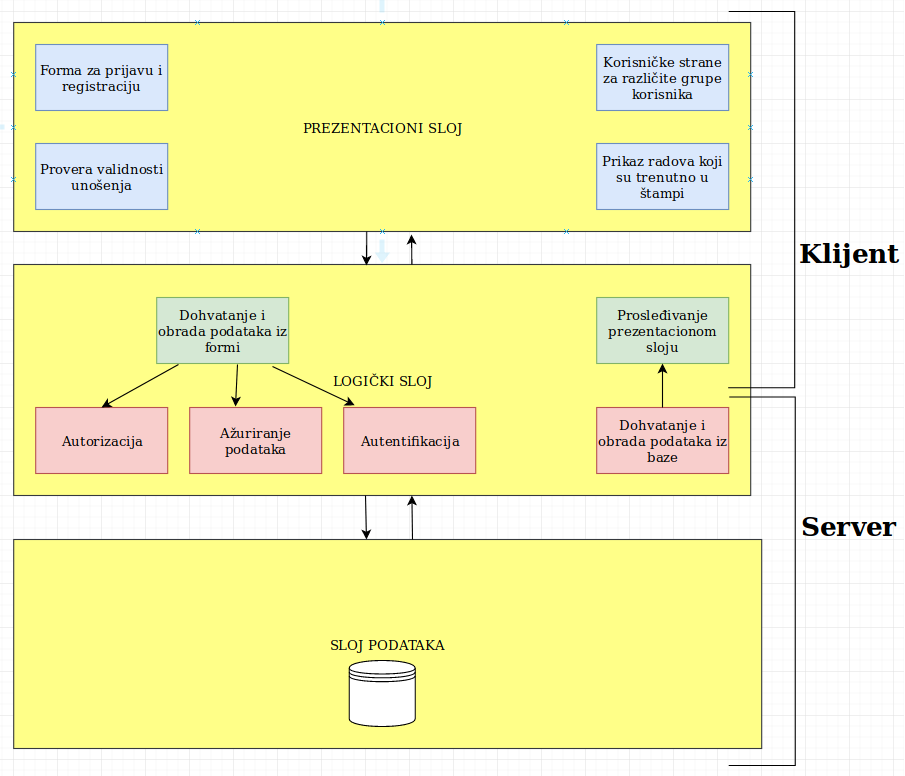
\includegraphics[scale=0.5]{Architecture.png}
    \caption{Troslojna arhitektura sa podeljenim logičkim slojem \cite{draw}}
    \label{fig:arhitektura}
\end{figure}
    
    Odabrana je \textbf{troslojna arhitektura} (slika \ref{fig:arhitektura}) zato što je:
    \begin{itemize}
        \item prilagodljiva brzim promenama u korisničkom i implementacionom okruženju
        \item jednostavna i intuitivna za implementaciju
        \item omogućava transparentno povezivanje korisnika sa izvorima podataka koji su im potrebni
    \end{itemize}
    
    \textbf{Prezentacioni sloj:}
    \begin{itemize}
        \item Forma za prijavu i registraciju
        \item Provera validnosti unošenja: Prilikom popunjavanja formi proverava se validnost podataka - u polje za email je unet ispravan email, sva obavezna polja su popunjena...
        \item Korisničke strane za različite grupe korisnika: različitim grupama korisnika se prikazuju različite korisničke strane
        \item Prikaz radova koji su trenutno u štampi
    \end{itemize}
    
    \textbf{Logički sloj:}
    \begin{itemize}
        \item Dohvatanje i obrada zahteva i podataka: Nakon dohvatanja zahteva i podataka iz formi, vrši se njihova obrada tako da budu spremni da prođu autorizaciju, autentifikaciju, ažuriraje podataka ili slanje zahteva
        \item Autorizacija
        \item Autentifikacija
        \item Ažuriranje podataka: obrađeni podaci se upisuju u bazu podataka (insert i update upiti)
        \item Slanje zahteva: zahtevi se šalju ka bazi podataka i od nje zahtevaju podaci (select upiti)
        \item Dohvatanje i obrada podataka iz baze: dohvataju se i obrađuju podaci koji su zahtevani select upitima
        \item Prosleđivanje prezentacionom sloju: obrađeni podaci se pakuju u oblik pogodan za prezentacioni sloj i time njemu prosleđuju
    \end{itemize}
    
    \textbf{Sloj podataka:} Predstavlja bazu podataka
    
\newpage

\addcontentsline{toc}{section}{Literatura}
\appendix
\bibliography{literatura} 
\bibliographystyle{plain}
    
\end{document}






















